% test citing
%\cite{CFried:Privacy}
%\cite{WarrenBrandeis:RightToPrivacy}
%\cite{sep-privacy}
%\cite{7ToP}
%\cite{Grimm:ItSecRefModel}
%\cite{ItSecGlossary}
%\cite{SociotechnicalArchitectureForOnlinePrivacy}
%\cite{EUDataProtectionDirective}
%\cite{EUConventionOnHumanRights}
%\cite{Bundesdatenschutzgesetz}
%\cite{Gutwirth:DefiningPrivacy}
%\cite{UKDataProtectionAct}

\chapter{Legal and Ethical aspects of Privacy}
\label{chap:privacy}

\newcommand{\om}{[...]\xspace} % omission
%\newcommand{\om}{\ldots} % omission

As privacy is a very general and hard to grasp term, we need to fix a definition of privacy that is suitable for our needs.
As background information we include an overview about historical treatments of privacy as well as legal regulation of privacy in the European Union.
Based on this we propose a definition of privacy as {\em control over personal data}, and introduce seven privacy types that give specify the term {\em personal data} in the context of mobile sensor data collection.

% \section{Histrocial Approaches to Privacy}

\section{Legal Aspects of Privacy}

In the following sections we outline the most relevant legislature regarding privacy protection,
from on European angle.
Of particular importance is the EU Directive 95/46/EC that is discussed in section \ref{EUDIR}.

Based on the legal background presented here, we will derive the legal privacy requirements for our systems in \ref{sec:LEGAL_REQ}.

\subsection{European Convention on Human Rights}

The \emph{Europen Convetion on Human Rights} \cite{ECHR} was created by the members of the \emph{Council of Europe} (CoE) in 1953 as part of the aftermath of the second world war.
It formulates universal rights of citizens against the state authority.
All member states of the Council of Europe, which includes all EU members, have incorporated this convention into their national law.

Article 8 of the ECHR contains a protection of personal data.

\begin{quote}
(1) Everyone has the right to respect for his private and family life, his home and his correspondence.

(2) There shall be no interference by a public authority with the exercise of this right except such as is in accordance with the law and is necessary in a democratic society in the interests of national security, public safety or the economic well-being of the country, for the prevention of disorder or crime, for the protection of health or morals, or for the protection of the rights and freedoms of others.
\end{quote}

The protection of personal data under Article 8 is not an absolute law but must be considered in relation to other laws such as the freedom of expression (ECHR, Art. 10).
The \emph{European Court of Human Rights} (ECtHR) overseas the implementation of this directive and has adopted a rather broad interpretation of the article.\footnote{\url{http://en.wikipedia.org/wiki/Article_8_of_the_European_Convention_on_Human_Rights}}

In particular State actions of searching a persons home, gathering and storing information in a secret police file, and stopping a prisoner's communication have been ruled to interfere with Article 8.

The Live+Gov systems can violate this fundamental human right if it is used to gather information about the private life without the knowledge and consent of the citizen.

% In the context of the Live+Gov project the ECHR is of limited relevance, since the Live+Gov System is offered by private companies and not directly by the State authority.

\subsection{OECD Guidelines and CoE Convention 108}

The emergence of information technologies that allow automated processing of personal data made more detailed rules for safeguarding the privacy of citizens necessary.
In the light of this developments the OECD  \cite{OECD80} issued Guidelines on Protection of Privacy in 1980 which establish the following basic principles of data protection:
\begin{enumerate}
\item Collection Limitation Principle.
  There should be limits to the collection of personal data and any such data should be obtained \om with the knowledge or consent of the data subject.
\item Data Quality Principle.
  Personal data should be relevant to the purposes for which they are to be used, and,  \om accurate, complete and kept up-to-date.
\item Purpose Specification Principle.
  The purposes for which personal data are collected should be specified \om and the subsequent use limited to the fulfillment of those purposes \om.
\item Use Limitation Principle.
  Personal data should not be disclosed \om except: a) with the consent of the data subject; or b) by the authority of law.
\item Security Safeguards Principle.
  Personal data should be protected by reasonable security safeguards \om.
\item Openness Principle.
  {\om} Means should be readily available of establishing the existence and nature of personal data, and the main purposes of their use, as well as the identity and usual residence of the data controller.
\item Individual Participation Principle.
  An individual should have the right
  \begin{itemize}
  \item to obtain from a data controller, or otherwise, confirmation of whether or not the data controller has data relating to him;
  \item to have communicated to him, data relating to him \om
  \item \om to have the data erased, rectified, completed or amended.
  \end{itemize}
\item Accountability Principle.
  A data controller should be accountable for complying with measures which give effect to the principles stated above.
\end{enumerate}

Where the following definitions are understood.
\begin{itemize}
\item \emph{personal data} means any information relating to an identified or identifiable person (\emph{data subject}).
  An identifiable person is one who can be identified either directly, by reference to a name or identification number or indirectly, by one or more factors which make it possible to find out who the data subject is by conducting further research.
\item a \emph{data controller} means any party who is competent to decide about the contents and use of personal data.
\end{itemize}

The OECD guidelines were adopted by EU law in the Strassbourg Convention 108 of the Council of Europe \cite{CONV108} in 1981.

Relevant for our investigations is in particular, that sensor data collected from mobile devices is considered personal data if the individual can be identified based on the data by any direct or indirect means.
Therefore the above principles apply.

% UPDATE 2013: http://www.oecd.org/sti/ieconomy/privacy.htm

\subsection{EU Data Protection Directive}\label{EUDIR}

The \emph{Directive 95/46/EC} of 1995 \cite{DIR95} is the fundamental regulation of data protection in the European Union.
It was designed to give further substance to the Convention 108.
In particular it makes the creation of an independent supervisory authority necessary (Art. 28).
As this text is the main legal basis for our investigation we review it in detail.
In Section \ref{sec:ECIMPL} the status of the implementation is discussed in some example cases.

The interpretation and oversight of the Directive lies at the Court of Justice of the European Union (CJEU).
A summary of the most important rulings can be found in Handbook on European data protection law \cite{EU_HANDBOOK_2014}.

The ambition of the Directive is stated at the very beginning.
\begin{quote}
  (Art. 1.1) In Accordance with this Directive the Member States shall protect the fundamental rights and freedoms of natural persons, and in particular their right to privacy with respect to the processing of personal data.
\end{quote}

The Directive follows the definition of personal data, data subject, and data controller of the OECD Guidelines (cf. Art. 2).
Furthermore it introduces the role of a \emph{processor} as a person which processes, by wholly or partly automatic means (Art 3.), personal data on behalf of the controller.

Data collection of intelligence agencies and the police is not restricted by the Directive (Art. 3).

The most important articles are summarized in the following paragraphs.
In order to keep the text more readable we have simplified the formulation by removing the formulation ``Member States shall provide that ...'' from each paragraph.
\begin{itemize}
\item (Art. 6.1.a) Personal data must be processed fairly and lawfully.

[The meaning of the term 'fair processing' is entailed in the following articles.
In particular transparency of processing, information of the data subject, and right to access the data are implied (cf. \cite{EU_HANDBOOK_2014})]

\item (Art. 6.1.b) \emph{Specification of Purpose.} Personal data must be collected for specified, explicit and legitimate purposes and not be processed in a way incompatible with this purposes.

Further processing of data for historical, statistical or scientific purposes shall not be considered incompatible \om.

\item (Art. 6.1.c) Personal data must be adequate, relevant and non-excessive in relation to the purposes \om.

\item (Art. 6.1.d) \emph{Accuracy.} Personal data must be accurate and \om every reasonable step must be taken to ensure that data which is inaccurate or incomplete \om are erased or rectified.

\item (Art. 6.1e) Personal data must be kept in a form which permits identification for no longer than is necessary \om.
% \item (Art. 6.2) It shall be for the controller to ensure that (Art. 6.1) is complied with.
\end{itemize}

In addition to strengthening the OECD Data Quality Principle in Article 6, the Directive requires a strong form of consent of the data subject, before any collection or processing of data can take place.

\begin{itemize}
\item (Art. 7). Personal data may be processed only if:
  \begin{itemize}
    \item [(a)] the data subject has unambiguously given his consent; or
    \item [(..)] [exceptions are made for performance of a contracts with the data subject,  legal obligations of the controller, to protect vital interests of the data subject, the public interest and]
     \item [(f)] the processing is necessary for purposes of legitimate interests pursued by the controller or by a third party to whom the data are disclosed, except where such interests are overridden by the interests \om of the data subject which require protection under Art. 1(1).
  \end{itemize}

\item (Art. 8.1) \emph{Special Categories.} Member Stats shall prohibit the processing of personal data revealing racial or ethnic origin, political opinions, religious or philosophical beliefs, trade-union membership, and the processing of data concerning health or sex life. [Art. 8.2 lists several exceptions, including explicitly explicit consent of the data subject.]
\end{itemize}

The OECD Participation Principle is addressed and extended in the following articles.

\begin{itemize}
\item (Art. 10, 11) The controller \om must provide a data subject \om with the following information:
  \begin{itemize}
    \item [(a)] the identity of the controller \om
    \item [(b)] the purpose of processing for which the data are intended;
    \item [(c)] any further information \om that is necessary to guarantee fair processing in respect of the data subject. [This includes in particular the recipients of the data, the existence of the right to of access and the right to rectify the data.]
  \end{itemize}

\item (Art. 12) \emph{Right to Access.} Every data subject has the right to obtain from the controller
\begin{itemize}
  \item (a) \om confirmation as to whether or not data relating to him are being processed \om, communication to him \om the data undergoing processing and any available information as to their source, knowledge of the logic involved in any automatic processing \om;
  \item (b) the rectification, erasure or blocking of data the procession of which does not comply with the provisions of this Directive \om;
  \item (c) notification to third parties to whom the data have been disclosed \om.
\end{itemize}

%\item Confidentiality of Processing (Art. 16).
%Any person under the authority of the controller or of the processor \om who has access to personal data must not process them except on instructions from the controller, unless he is required to do so by law.
\end{itemize}

A similar form of the Security Safeguard Principle is contained in Article 17.

\begin{itemize}
\item (Art. 17) \emph{Security of processing.}
The controller must implement appropriate technical and organizational measures to protect personal data against accidental loss, alteration, unauthorized disclosure or access \om and against all other forms of unlawful processing.

[The level of security has to be balanced against the risk of processing.]

% Having regard to the state of the art and the cost of their implementation, such measures shall ensure a level of security appropriate to the risk represented by the processing and the nature of the data to be processed.
\end{itemize}

Furthermore the Directive demands all data processing to be reported to a supervisory authority.
This obligation can be lifted if an internal data protection official is appointed, who is responsible in particular for keeping a processing register, that has to be made available on request.

\begin{itemize}
\item Notification (Art. 18. 1).
The controller \om must notify the supervisory authority referred to in Article 28 before carrying out any wholly or partly automatic processing operation \om.

\item (Art. 18.2).
Simplification or exemption from notification may be provided only under the following conditions: \om where the controller \om appoints a personal data protection official, responsible in particular:
\begin{itemize}
\item for ensuring in an independent manner the internal application of the national provisions taken pursuant to this directive.
\item for keeping the register of processing operations carried out by the controller, containing the items of information referred to in Article 21 (2)
\end{itemize}
thereby ensuring that the rights and freedoms of the data subjects are unlikely to be adversely affected by the processing operations.

\item (Art. 19.1)
The information to be given in the notification shall include at least:
\begin{itemize}
  \item [(a)] the name and address of the controller \om;
  \item [(b)] the purpose \om of processing;
  \item [(c)] a description of the category \om of the data \om;
  \item [(d)] the recipients \om to whom the data might be disclosed;
  \item [(e)] proposed transfer of data to third countries;
  \item [(f)] a general description allowing a preliminary assessment to be made of the appropriateness of the measures taken pursuant of Article 17 to ensure the security of processing;
\end{itemize}

\item (Art. 21.2) \emph{Publication}.
A register of processing information \om shall be kept at the supervisory authority.
The register shall contain at least the information listed in Article 19.1 (a) to (e).

The register may be inspected by any person.

\item (Art. 21.3). In relation to processing operations not subject to notification, that controllers \om make available at least the information referred to in Article 19.1 (a) to (e) in an appropriate form to any person on request.

\item (Art. 28) \emph{Supervisory Authority.}
Each Member State shall provide that one or more public authorities are responsible for monitoring the application \om of this Directive.

These authorities shall act in complete independence in exercising this functions entrusted to them.
\end{itemize}

Data transfer to third countries outside of the EU requires those countries to have an adequate level of data protection.
\begin{itemize}
\item (Art. 25.1) \emph{Transfer to third countries.}
The transfer to a third country of personal data \om may take place only if \om the third country in question ensures an adequate level of protection.
\end{itemize}
The European Commission can decide whether a third country ensures an adequate level of protection (Art 25.6).
The USA, is not considered to do so.
Data exchange between the US and EU is possible under the Safe Harbor regulation \cite{SAFE_HABOR}.
Further Exceptions are provided by the Passenger Name Record Agreement \cite{PNR}.

\subsection{Implementation of the Data Protection Directive}\label{sec:ECIMPL}

\textbf{Germany}.
Germany implements Directive 95/46 with the \emph{Bundesdatenschutzgesetz (BDSG)}
of 2001. However, Germany has violated the directive in two points:
\begin{enumerate}
\item The BDSG has become effective three years too late, thus the EC filed a treaty violation proceeding against Germany.
\item The BDSG does not implement independent supervisory authorities.
The Bundesdatenschutzbeauftragter is subordinate to the Ministry of Interior.
Although he is not subject to technical oversight (\emph{Fachaufsicht}), he is subject to staff supervision by the government (Rechtsaufsicht, Dienstaufsicht) and budget oversight by the ministry.
In March 2010 Germany was found guilty of violation of Directive 95/46 by the ECJ.
\end{enumerate}

The states of Germany have their own implementation of Directive 95/46 (\emph{Landesdatenschutzgesetze}).
Federal public authorities are only bound to their federal law.
Churches are not subject the BDSG.

\textbf{United Kingdom.}
The UK implements Directive 95/46 with the \emph{Data Protection Act 1998} (DPA).

%TODO: Reformulate Wikipedia Text

%% The act is known for its high complexity: a manual record of phone numbers for business purposes could be hold subject to the DPA.
%% Although the act seems to fully cover the directive.
%% Even higher restriction apply for \emph{``sensitive personal data''} (race, ethnicity, politics, religion, trade union status, health, sex life or criminal record), i.e. consent must be given freely and has to be explicit.

%% The Act's definition of personal data covers any data that can be used to identify a living individual.
%% Anonymised or aggregated data is not regulated by the Act, providing the anonymisation or aggregation has not been done in a reversible way.

%% The Freedom of Information Act 2000 modified the act for public bodies and authorities, and the Durant case modified the interpretation of the act by providing case law and precedent.

%% The Data Protection Act creates rights for those who have their data stored, and responsibilities for those who store, process or transmit such data.
%% The person who has their data processed has the right to:
%% \begin{itemize}
%% \item View the data an organization holds on them.
%% A `subject access request' can be obtained for a nominal fee.
%% As of January 2014, the maximum fee is \pounds2 for requests to credit reference agencies, \pounds50 for health and educational request, and \pounds10 per individual otherwise.
%% \item Request that incorrect information be corrected.
%% If the company ignores the request, a court can order the data to be corrected or destroyed, and in some cases compensation can be awarded.
%% \item Require that data is not used in any way that may potentially cause damage or distress.
%% \item Require that their data is not used for direct marketing. \cite{3}
%% \end{itemize}


\textbf{United States of America}
The USA do not implement the directive, nor is there any obligation for them to do so.
However, companies subject to US jurisdiction can be certified to comply with the seven principles enforced by Directive 95/46.
Thus, those companies will act as \emph{safe harbors}.
Without certification foreign companies are not allowed to store and process customer data in their country.


\subsection{EU Charter of Fundamental Rights}
The Treaty of Lisbon of 2007, which introduced the fundamental functioning of the European Union
includes the \emph{Charter of Fundamental Rights of the Europen Union} \cite{EUFR2010}.
This Charter summarizes the full range of civil, political and economic rights of EU citizens and contains the following two articles that safeguard the privacy of the citizen.

\begin{quote}
  Article 7. Respect for private and family life.\\
  Everyone has the right to respect for his or her private and family life, home and communications.

  Article 8. Protection of personal data.
  \begin{enumerate}
    \item [(1)] Everyone has the right to the protection of personal data concerning him or her.
    \item [(2)] Such data must be processed fairly for specified purposes and on the basis of the consent of the person concerned or some other legitimate basis laid down by law.
      Everyone has the right of access to data which has been collected concerning him or her, and the right to have it rectified.
    \item [(3)] Compliance with these rules shall be subject to control by an independent authority.
  \end{enumerate}
\end{quote}

Although the Charter does not extend the pre-exiting Directive 95/46/EC, it amplifies the importance of this privacy protection as a fundamental right.

\section{Privacy Definition and Taxonomy}
\label{sec:taxonomy}

\subsection{Defining Privacy}

% TODO: Expand this section!!

Defining privacy is a challenge which seems impossible. This is well put to words by Serge Gutwirth, who notes:

\begin{quote}
The notion of privacy remains out of the grasp of every academic chasing it. Even when it is cornered by such additional modifiers as `our' privacy, it still finds a way to remain elusive. \cite{Gutwirth}
\end{quote}

%Many researchers seem to only ``focus on the ways in which privacy can be infringed'' \cite{7ToP}.
%Thus they try to create taxonomies of \emph{privacy harms} instead of taxonomies of \emph{privacy types}.
%Those two differ in the respect that the former focuses on threats to prohibit whereas the latter focuses on values to protect.
%So one should rather evaluate what aspects are precious about privacy and develop measures to ensure their security than only forbid single actions against it \cite{7ToP}.

Many researchers seem to only ``focus on the ways in which privacy can be infringed'' \cite{7ToP}.
Thus they invest a great amount of work in defining threats to prohibit instead of describing why privacy is so valuable to us.
This way around one could derive measures to ensure and secure its value \cite{7ToP}.
One particular scholar who does this in the context of digital monitoring is Charles Fried.
He questioned, why we are intuitively sensitive to violations of privacy.
But he did not assert privacy as an intrinsic value by itself, he rather sated:

\begin{quote}
Privacy is not simply an absence of information about us in the minds of others;
rather it is \textbf{the control we have over information about ourselves}. \cite{CFried:Privacy}
\end{quote}

According to Fried privacy is a \textit{rational context}.
Which means that one is aware of such context's existence during a rational action.
If we are to share private information with others, we are most likely aware that this action is privacy related.
In that case we are able to selectively disclose information along the two dimensions of quantity and quality.
This leads Fried to his thesis, that privacy is one's ability to create and modulate his or hers social relationships, namely: friendship, love and trust. \cite{CFried:Privacy}

Depending on the conversation partner, we change the degree of intimate information we share if it is a total stranger, colleague, close friend or lover.
With close friends or lovers we share information of great intimacy we do not share with anyone else.
Moreover, we trust those persons to not reveal information about us to others by respecting their privacy.
Trust needs the possibility of unknown failure.
If we would constantly monitor our partners, they cannot fail unnoticed nor can they willingly share that information with us.
Thus they could not trust us anymore. \cite{CFried:Privacy}

So privacy or the its possibility, according to Fried, is the foundation of our core relations: friendship, love and trust.
And thus it is valuable, because those relations are essential to human society \cite{CFried:Privacy}. 
Using his anatomy of privacy as foundation of our analysis is suitable because of two points.
At first, Fried's study on the understanding of privacy provided a great contribution to the research on the same term in philosophy \cite{sep-privacy} and computer science \cite{SociotechnicalArchitectureForOnlinePrivacy}.
Secondly, despite the fact his text was published in 1970, he already included technologies to its viewpoint that did not only monitor location, but also record biometric data.

%TODO: Iterate Section. Exmplain Triangular Relationship:
- Subject
- Trusted Person
- Third Party which shall NOT obtain sensitive information.

\subsection{The Seven Types of Privacy}

Although we use Fried's definition of privacy as one's control over information about oneself, we do not feel safe conducting a privacy protection analysis relying only him.
We need additional means to analyze in more detail which aspects of our lives need protection.
Friedewald, Finn and Wright \cite{7ToP} introduced a privacy taxonomy called \textit{Seven Types of Privacy} that can be of help.
The seven types of privacy are an extension to the four types of privacy by Roger Clarke \cite{RClarke:4ToP}:
\begin{itemize}
\item Privacy of the Person
\item Privacy of Personal Behaviour
\item Privacy of Personal Communication
\item Privacy of Personal Data
\end{itemize}
However, Friedewald et al. felt that Clarke's taxonomy is technologically outdated and no longer adequate.
In order to fix this they extend the former four to the now introduced seven types privacy as follows:

\begin{enumerate}

\item \textbf{Privacy of the Person}

This privacy type is generally concerned with one could best understand as biometric privacy. 
Friedewald et al. paraphrase it as \emph{``\om the right to keep body functions and body characteristics \om private''}. 
This includes but is not limited to measures like weight, height or shoulder width;
biometric identifiers like fingerprints and DNA sequences;
or medical conditions such as limping or having a cold. \cite{7ToP}


\item \textbf{Privacy of Behaviour and Action}

This privacy type is concerned with one's activities in public as well as in private spaces. 
It includes but is not limited to religious practices, political activities and sexual preferences or habits. \cite{7ToP}


\item \textbf{Privacy of Communication}

This privacy type is concerned with one's communication in a broad sense.
It includes written correspondence, but also conversations conducted either vis-a-vis or via electronic devices.
Friedewald et al. put it as the right to free discussion without unknown interception by third parties. \cite{7ToP}


\item \textbf{Privacy of Data and Image}

This privacy type is concerned with the secrecy of one's personal data, especially its automatic disclosure to other individuals and organizations.
It includes data such as paychecks, insurance information or records of public administration.
However, it also refers to pictures taken without consent and digital identifiers like IP addresses or social security numbers. \cite{7ToP}


\item \textbf{Privacy of Thoughts and Feelings}

This privacy type is the counterpart to Privacy of the Person like body and mind are counterparts of one another.
Comparable to the Privacy of Data and Image, Friedewald et al. state that one's thoughts and feelings must not be automatically revealed to others.
This could simply happen by the disclosure of one's diary or by technologies which allow emotion detection through biometric means.
One's body temperature or iris reflexes might infer stress or excitation. \cite{7ToP}


\item \textbf{Privacy of Location and Space}

This privacy type is concerned with one's movements in public spaces and the inviolateness of one's private spaces.
Friedewald et al. qualify the first dimension as one's right to move without being identified, tracked or monitored.
The second dimension is qualified as one's general right to solitude, especially the right to the inviolability of the home. \cite{7ToP}



\item \textbf{Privacy of Association}

This privacy type is also put as group privacy.
Friedewald et al. state that one must have the possibility with whomever without being recorded.
Associations like friends or organizations such as political parties must not automatically  be recorded because one associates with them, and vice versa.

\end{enumerate}

\subsection{Privacy Type Inferences}

The above types of privacy types are not disjoint to each other.
For example if the location of a citizen is known it is possible to infer information about political associations (e.g. his visits to a party meeting).
In this section we explore possibilities how personal data can be inferred from each other.
Our findings are summarized in Figure \ref{figure:Implicit Privacy Violation Matrix}.

%\includegraphics{../diagrams/png/implicit-privacy-violation-matrix.png}
\begin{figure}
\centering
\includegraphics[width=\textwidth]{diagrams/png/implicit-privacy-violation-matrix.png}

\begin{flushleft}
\scriptsize
\textbf{Legend:}
The matrix above shows the following relation: \emph{Type X can be
implicitly violated by the violation of type Y.}
\begin{itemize}
\itemsep1pt\parskip0pt\parsep0pt
\item
  The X-Axis shows the Seven Types of Privacy according to Friedewald et
  al., which could be violated implicitly
\item
  The Y-Axis shows the Seven Types of Privacy according to Friedewald et
  al., which have been violated explicitly
\item
  Big black bullet points denote, that an implicit violation is possible
\item
  Big grey bullet points only denote, that the relation is reflexive
  (\emph{a R a}). They are only shown for completeness sake and not
  discussed further, because they denote a trivial fact.
\end{itemize}
\end{flushleft}

\caption{Implicit Privacy Violation Matrix}
\label{figure:Implicit Privacy Violation Matrix}
\end{figure}


\paragraph*{1. Privacy of The Person}

The Privacy of The Person is concerned with one's biometric privacy.
If this type is violated, following implicit violations are possible:

\begin{itemize}
\item [(1-5)]
  Privacy of Thoughts and Feelings. Some psychological diseases
  (e.g.~depression) have physiological impact. Such physiological
  patterns could be detected.
\end{itemize}

\paragraph*{2. Privacy of Behaviour and Action}

The Privacy of Behaviour and Action is concerned with one's social, political, religious, sexual, etc. activities.
If his type is violated, following implicit violations are possible:

\begin{itemize}
\item [(2-1)] Privacy of The Person.
  Religious practices which include body modifications (e.g.~circumcision).
\item [(2-5)] Privacy of Thoughts and Feelings.
  Social activities in general depend on a certain intellectual attitude.
  Such an activity is the expressions of such an attitude.
\item [(2-7)] Privacy of Association.
  Recording religious, political or sexual activities can reveal association with churches, political parties or sexual partners.
\end{itemize}

\paragraph*{3. Privacy of Communication}

The Privacy of Communication is concerned with not having such communication (correspondence or vis-a-vis) intercepted.
This is very broad type of privacy.
Depending on the contents of the intercepted communication every other type can be violated:

\begin{itemize}
\item [(3-1)] Privacy of The Person. Communication about body characteristics.
\item [(3-2)] Privacy of Behaviour and Action. Communication about social activities.
\item [(3-4)] Privacy of Data and Image.
  Communication containing one's passwords or other sensitive data.
\item [(3-5)] Privacy of Thoughts and Feelings.
  Communication of thoughts and feelings, e.g.~wiretapping a flirt or a catholic confession
  ritual.
\item [(3-6)] Privacy of Location and Space.
  Interception of face-to-face communication is only possible if one's location and space is violated (wiretapping).
\item [(3-7)] Privacy of Association.
  Communication about one's associations (family members, churches, etc.).
\end{itemize}

\paragraph*{4. Privacy of Data and Image}

The Privacy of Data and Image is concerned with one's data not being automatically available to others.
This also is a very broad type of privacy.
Depending of the data or image contents every other type can be violated:

\begin{itemize}

\item [(4-1)] Privacy of The Person.
  Images or stored biometric information reveal one's physical characteristics.
\item [(4-2)]Privacy of Behaviour and Action.
  Images or diaries can reveal one's social activities.
\item [(4-3)]Privacy of Communication.
  Modern communication systems usually contain some sort of archive function, e.g.~E-mail clients do not automatically delete messages.
  Such messages are data and reveal one's communication.
\item [(4-4)]Privacy of Thoughts and Feelings.
  Images can show one's emotional state.
\item [(4-5)]Privacy of Location and Space.
  Images can reveal one's location, e.g.~making a picture in front of the Eifel Tower.
\item [(4-6)]Privacy of Association. E-mail data can also reveal
  association.
\end{itemize}

\paragraph*{5. Privacy of Thoughts and Feelings}

The Privacy of Thoughts and Feelings is concerned with keeping such
thoughts and feelings secret. If this type is violated, following
implicit violations are possible:

\begin{itemize}
\item [(5-1)] Privacy of The Person.
  Thoughts and feelings can reveal medical conditions.
\item [(5-2)] Privacy of Behaviour and Action.
  Thoughts and feelings can reveal a certain attitudes which create a foundation for certain   social activities.
\item [(5-7)] Privacy of Association.
  Thoughts and feelings can reveal individual association, e.g amorous feelings for a certain person.
\end{itemize}

\paragraph*{6. Privacy of Location and Space}

The Privacy of Location and Space is concerned with one's right to move freely without being tracked and one's right to private places.
If this type is violated, following implicit violations are possible:

\begin{itemize}
\item [(6-1)] Privacy of The Person.
  Frequently visited doctors can reveal certain medical conditions, if such doctors are known specialsts.
  In general it could imply illness.
\item [(6-2)] Privacy of Behaviour and Action.
  Frequently visited places in general can reveal association and hence implies social activities.
\item [(6-3)] Privacy of Communication.
  If one's location is knwon, it is possible to intercept (wiretap) one's communication.
  This also may violate the right to private spaces.
\item [(6-4)] Privacy of Data and Image.
  If one's location is known, it is possible shoot pictures.
\item [(6-5)] Privacy of Thoughts and Feelings.
  Frequently visited persons may imply certain thoughts and feelings, e.g.~having a mistress.
\item [(6-6)] Privacy of Association.
  Frequently visited places can reveal associations simply by searching in maps or yellow-pages.
\end{itemize}

\paragraph*{7. Privacy of Association}

The Privacy of Association is concerned with one's right to associate with whomever one wants, without that association having recorded.
If this type is violated, following implicit violations are possible:

\begin{itemize}

\item [(7-1)] Privacy of The Person.
  Association with tattoo artists could imply having tattoos or other body modifications.
\item [(7-2)] Privacy of Behaviour and Action.
  Association with churches or political organizations could imply certain activities.
\item [(7-5)] Privacy of Thoughts and Feelings.
  Association with churches of political organizations could imply a certain intellectual attitude.
\end{itemize}




%%%%%%%%%%%%%%%%%%%%%%%%%%%%%%%%%%%%%%%%%%%%%%%%%%%%%%%%%%%%%%%%%%%%%%
%%%%%%%%%%%%%%%%%%%%%%%%%%%%%%%%%%%%%%%%%%%%%%%%%%%%%%%%%%%%%%%%%%%%%%
%%%%%%%%%%%%%%%%%%%%%%%%%%%%%%%%%%%%%%%%%%%%%%%%%%%%%%%%%%%%%%%%%%%%%%

\pagebreak

\chapter{Privacy Analysis of Live+Gov Systems}

The goal of this chapter to analyze and identify the threads to personal privacy that are posed by collecting, storing and processing sensor data from mobile phones.
We derive concrete privacy protection measures that address the main risks involved with handling such data.

The complexity of our systems and the variety of threads make a great number of counter measures plausible.
We approach this complexity with the aid of a general security analysis model developed in \cite{Grimm:ItSecRefModel}.
We give a brief introduction to this model and perform a IT Security Analysis with respect to the privacy asset for our system.

\section{IT Security Analysis according to Grimm et. al}

We follow the Reference Model for IT Security Analyis as described in \cite{Grimm:ItSecRefModel}.
It supersedes earlier efforts by \cite{Avizienis}.

The reference model consists of a \emph{model} and a \emph{procedure}.
The model aims to organize common security terminology in a reasonable and practical way.
The procedure describes a method to analysis the IT system based on that model.
In this section we give a brief overview over the reference model.

\subsection{Model}

%\includegraphics{../diagrams/png/itsec-ref-model-grimm.png}
\begin{figure}
\centering
\includegraphics[width=\textwidth]{diagrams/png/itsec-ref-model-grimm.png}
\caption{The IT Security Reference Model (Grimm)}
\end{figure}


The model is depictured in Figure \ref{fig:refmodel}.
It is organized in four views (round boxes) that contain a number of components (rectangular boxes).

%%%%%%%%%%%%%%%%%%%%

The \emph{world view} contains all components describing the current state.
It consists of the following components:
\begin{itemize}
\item \textbf{Actors.}
All identifiable stakeholders of the system under study.
Typical actors include, users, developers, clients and externals.

\item
\textbf{Assets.} Things of value to one or more stakeholders.
The value can be hard (money, data, etc.) or soft (trust, privacy,etc.).
In our case the only asset we are concerned with is the privacy of the citizen.

\item \textbf{IT-Systems.}
The relevant IT-Systems under study. This encompasses hardware (e.g. servers, network infrastructure), as well as software and third party services.
The level of granularity has to be detailed enough to express all possible threats to the assets at stake.

\item \textbf{Conflicts of Interests.}
Different actors have different interests which can be in conflict which each other.
These conflicts of interest are the origin of all attacks to the system.

A typical conflict is the \emph{Criminal-User-Conflict}:
A user wants to keep control over their private data.
A criminal wants to gain money.
The possibility of selling private data (user profiles) to advertisers, renders both interests conflicting.

\item \textbf{Vulnerabilities.}
All identifiable weaknesses in the IT-System.

In the example of the criminal-user-conflict, the criminal has to exploit a vulnerability, e.g. a weak password, to gain access to the private data about the user.

\item \textbf{Interactions.}
This point captures all possible interactions between assets, IT-Systems, humans and vulnerabilites.
It is described in more detail in the next view.
\end{itemize}


%%%%%%%%%%%%%%%%%%%%


The \emph{potential view} displays the intended and unintended interactions of the components in the world view.
The intended interactions support the underlying business objectives.
Unintended interactions lead to threats.
The potential view consists of the following components.
\begin{itemize}
\item \textbf{Business Objectives.}
Interaction of IT-system and actors that realize a business goals of the system owner.

\item \textbf{Threats.}
A threat is a potential interaction that destroys or harms assets of the system.
Concrete realizations of threats can be \emph{attacks} or \emph{accidents}.
Attacks are executed by an actor in response to a conflict of interest.
Accidents are harmful interactions that are not willfully caused by an actor.

\item \textbf{Chances/Risk.}
Evaluation of chances and risks associated to the business objectives and threats.
The risk associated to a threat is its expected loss.
A chance associated to a intended interaction is its expected gain.

In the case that, the loss can be quantified monetary, and the likelihood of occurrence of a threat can
be modeled probabilistically, the risk is given by the product
\[ \text{risk} = \text{loss} \cdot P[\text{threat}]. \]
In practice such a quantitative risk evaluation is often not possible, and a qualitative, heuristic, analysis is performed instead.

\item \textbf{Security Requirements.}
A set of interactions (e.g. threats) that shall not occur within the system in order to achieve its business objectives.
Security requirements are targeted to protect one or more assets.

An example of a security requirement is that a given communication channel shall not be infringed by externals.
\end{itemize}


%%%%%%%%%%%%%%%%%%%%


The \emph{concept view} is a realization of the potential view of the system.
It specifies important interactions that require further planning.
It contains the following components:
\begin{itemize}
\item \textbf{Business Model.}
The plan to achieve business objectives.

\item \textbf{Accident Scenario.}
A concrete outline of an interaction that leads to an accident.
In particular the asset under threatened and exploited vulnerability need to be described.

\item \textbf{Attack Technique.}
A specific technique or technology to attack IT-Systems (Man in the Middle, Phishing, etc.).
In particular the attacking actor, the conflict of interest and the exploited vulnerability need to be described.

\item \textbf{Security Measures.}
It describes a plan of sufficient measures to secure the intended interactions and to avoid the unintended interactions.
Each security measure targets a vulnerability of the system in order to reduce a risk for a certain thread.
\end{itemize}


%%%%%%%%%%%%%%%%%%%%


The \emph{event view} contains all actual events through out the lifetime of the system.
The event view instantiates the concept view of the system.
It contains the following components:
\begin{itemize}
\item \textbf{Business Process.}
The actual, running instance of the business model.

\item \textbf{Accidents.}
All actually happened accidents.

\item \textbf{Attacks.}
All actually happened attacks.

\item \textbf{Security Operations.}
Instances of security measures.
\end{itemize}


\subsection{Procedure}

The analysis procedure is an incremental and iterative process following the four views of the previously described model.

%\includegraphics{../diagrams/png/itsec-ref-model-grimm-procedure.png}
\begin{figure}
\centering
\includegraphics{diagrams/png/itsec-ref-model-grimm-procedure.png}
\caption{The IT Security Reference Analysis (Grimm)}
\end{figure}


\paragraph*{Step 1. World Analysis}

At first, one has to outline the current state of the system under study. This includes description of:
\begin{itemize}
\item all \textbf{Assets} which must be protected
\item all relevant \textbf{IT-Systems}
\item all involved \textbf{Humans} and their \textbf{Conflicts of Interests}
\item all known \textbf{Vulnerabilities}
\item and all important \textbf{Interactions} between the former components.
\end{itemize}

\paragraph*{Step 2. Potential Analysis}

Secondly, one needs to outline the potential interactions of the system under study.
This includes both the unintended interactions (threads) and the intended interactions (business objectives).
This step produces four artifacts:
\begin{itemize}
\item a \emph{threat specification}, which identifies the threat, its targeted assets, the involved actors and their conflicts of interest.
\item a \emph{threat risk evaluation}, which quantifies the likelihood of a threat manifestation in relation to its associated loss.
\item a \emph{security requirement specification}, which specifies requirements in order to deal with identified hazards
\end{itemize}

\paragraph*{Step 3. Concept Development}

Based on \textbf{Step 2.}, the identified hazards are used alongside realistic accident scenarios and attack techniques to create a \emph{risk matrix}.
With this matrix it is possible to decide if the risk is acceptable or not.
Together with the previously specified security requirements, the matrix is used to define adequate security measures.
Like a business model is an abstract concept to achieve business objectives, this step creates an concept to improve the system's security.

\paragraph*{Step 4. Concept Deployment}

Finally, the security measures have to be implemented.
Additionally, all business operations, accidents, attacks and executed security operations will be recorded in the following time.

The implementation of security measures changes the world view (e.g. IT-systems, actors) and renders the conducted analysis outdated.
So this analysis procedure needs to be conducted again.

\subsection{Abstraction Levels of the Reference Model}

The Reference Model can be used on different levels of abstraction.
This means each component can be used within a wide range of granularity, for instance the security measure \emph{Encryption} can be explored in general or on the level of different concrete encryption tools; or on the even finer level of concrete algorithms.

The utilized abstraction level is not important for the analysis procedure, it depends on the intended audience for the analysis.
However, it is important to use one abstraction level consistently through out the analysis.


%%%%%%%%%%%%%%%%%%%%%%%%%%%%%%%%%%%%%%%%%%%%%%%%%%%%%%%%%%%%%%%%%%%%%%%%%%%%%%%%%
%%%%%%%%%%%%%%%%%%%%%%%%%%%%%%%%%%%%%%%%%%%%%%%%%%%%%%%%%%%%%%%%%%%%%%%%%%%%%%%%%
%%%%%%%%%%%%%%%%%%%%%%%%%%%%%%%%%%%%%%%%%%%%%%%%%%%%%%%%%%%%%%%%%%%%%%%%%%%%%%%%%
\pagebreak

\section{Live+Gov Privacy Protection Analysis}

\subsection{Step 1. World Analysis}

\subsubsection{Assets: Privacy}

In this document we focus our attention to only one asset: The privacy of the citizen.

%TODO: UPDATE
Our definition of privacy is described in detail in Chapter \ref{chap:privacy}. In Section \ref{sec:taxonomy} we define privacy as the ``control over private data'' and introduce the following seven different types of privacy:
\begin{enumerate}
\item Privacy of the Person
\item Privacy of Behaviour and Action
\item Privacy of Communication
\item Privacy of Data and Image
\item Privacy of Thoughts and Feelings
\item Privacy of Location and Space
\item Privacy os Association
\end{enumerate}

Please refer to Section \ref{sec:taxonomy} for more details.

\subsubsection{IT-Systems \& Interactions}
\label{subsubsection:it-systems}

This section outlines the general architecture (Figure \ref{figure:IT Systems}) of IT systems for public monitoring comparable to the Live+Gov project.
This includes a description of it technical infrastructure and the interactions between its components.

The IT infrastructure of the Live+Gov system, i.e. the Live+Gov toolkit and the customization of the software components are described in detail in various project deliverables: D4.1, D4.3, D1.1, D5.1.
In this section we give an abstraction of those systems from the perspective of WP1.

\begin{figure}[h]
\centering
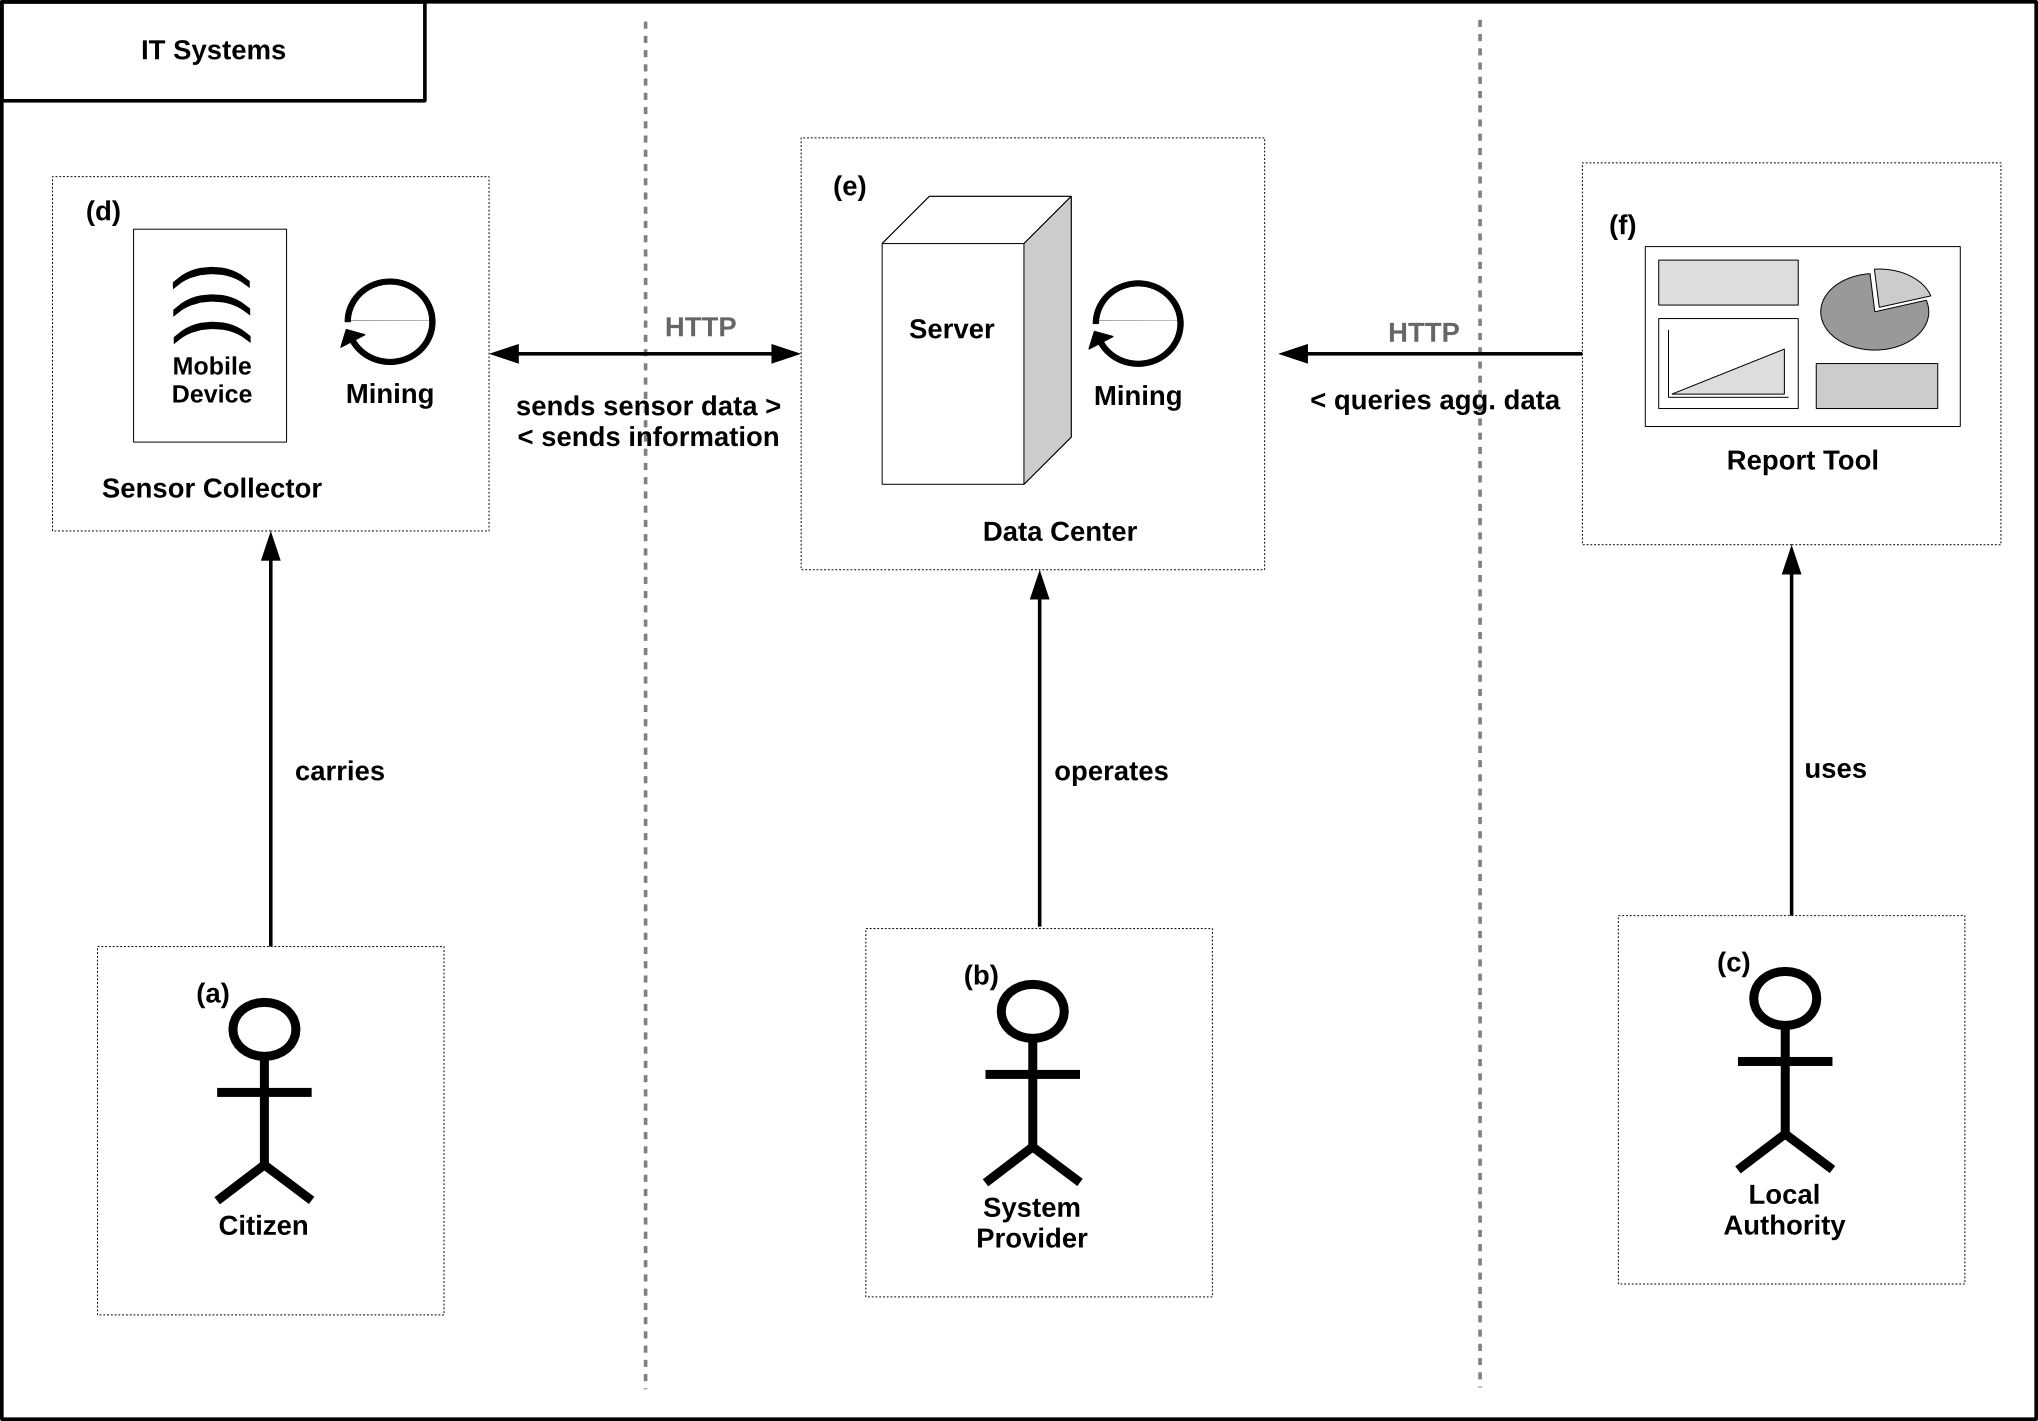
\includegraphics[width=\textwidth]{diagrams/png/it-systems.png}

\begin{flushleft}
\scriptsize
\textbf{Legend:}
\begin{itemize}
\itemsep1pt\parskip0pt\parsep0pt

\item
\textbf{(a) Citizen:} 
User of the L+G client application whose privacy is at stake.

\item
\textbf{(b) System Provider:} Provides technical infrastructure.

\item
\textbf{(c) Local Authority:} Provider of the L+G system.

\item
\textbf{(d) Mobile Device:}
Runs the L+G client application, produces and stores data sensitive to the users privacy.

\item
\textbf{(e) Data Center:} Runs the L+G services, processes and stores user data.

\item
\textbf{(f) Report Tool:} Interface to aggregated user data.

\end{itemize}
\end{flushleft}

\caption{IT Systems}
\label{figure:IT Systems}
\end{figure}


A \emph{citizen} (a) carries a mobile device running the \emph{sensor collector} application (d).
The sensor collector application is able to collect various kinds of sensor data (accelerometer, GPS, GSM, ...) and can sent the raw data back to the \emph{data center} (c).
The sensor collector can also be able to perform certain data mining operations.

Examples of such data mining operations include human activity recognition,the detection of service lines, detection of characters and faces from images.

In the Live+Gov Project mobile devices are used in particular for the following activities:
\begin{enumerate}
\item collection of GPS samples,
\item mining of Human activities (HAR) based on accelerometer samples,
\item collection of reports consisting of an image, free text and selected categories.
\end{enumerate}

The \emph{data center} stores and processes sensor data collected with the sensor collector application. It can also take into account data obtained from third parties, like the current positions of trains.
The data center can sent mining end products (traffic jam reports, bus schedule) back to the mobile device of the citizen.

In the Live+Gov Project data centers, in particular, perform the following activities:
\begin{enumerate}
\item storage of login credentials, name, and email address for each citizen,
\item storage of collected GPS samples (user id, timestamp, GPS location),
\item storage of HAR results (user id, timestamp, HAR result),
\item detection of service lines based received GPS samples (SLD),
\item storage of SLD results (userid, timestamp, SLD result),
\item sent back SLD results to mobile device,
\item storage of received reports (user id, timestamp, report),
\item detection of inherent patterns of the received reports.
\end{enumerate}

The \emph{System Provider} (b) provides and operates technical infrastructure like the Data Center and the \emph{Reporting Tool} (f).
The Reporting Tool queries the Data Center for aggregated data to visualize in form of charts and other means suitable to help understanding of monitored citizens.

\textit{Local Authorities} (c) use the reporting tool to get information in order to understand citizen movement and improve public services.
In such systems, the most valuable information for local authorities is not the raw sensor data, but aggregated views on the mining end products.

In the Live+Gov Project the reporting tools allows, in particular the following queries:
\begin{enumerate}
\item show aggregate information about which routes citizens take starting from a given location,
\item show the average waiting time of a citizen for each bus stop,
\item show routes where citizens where running to catch a bus,
\item show locations of all reports in a given time window,
\item visualize detected patterns in the report data,
\item view individual reports.
\end{enumerate}

\subsubsection{Actors}
\label{subsubsection:humans}

This section describes the human actors previously introduced within the IT system architecture (\ref{subsubsection:it-systems}).
Also the additional actor \textit{External} is introduced as a person with no special access rights.

\textbf{Citizen.}
Citizens are persons who use the mobile device as users of the provided software.
Their main motivation for using the software is to gain a higher level of convenience in their daily activities. For example they may have access to real time bus schedules or reports about traffic jams, that help them to avoid long waiting times.
Also they generally benefit from improvements of public infrastructure by local authorities, which is triggered by issue reports.

By using the application citizens are sharing personal information like name and address, as well as data gathered from mobile sensor with the service provider.
This data can be exploited in ways that are harmful to the citizen.
This need to protect this protection is manifest in several laws and constitutions as the right to privacy and data protection.
The citizen has a vital interest in having his legal rights protected and enforced.

If the right to privacy is violated, there is a magnitude of potential harms that interfere with other interests of the citizen.
This includes just annoying spam, where their technical identity is used to send unwanted commercials.
More severe phishing attacks can exploit personal information, and try to manipulate citizens into disclosing credentials like TAN numbers and disrespect their financial interests.
Information about the current location (GPS) or frequently used routes (stalking) can be used to attack and directly harm the health of the citizen.
Information about medical conditions inferred by sensor data (e.g. fintness trackers) are of interest to insurance companies, which may affect the pricing of policies and can interfere with financial interests of the citizen.

Also it is well established (cf. \cite{GuardienMassSurveillance}) that the very act of being monitored can have impact on mental health and performance, promotes distrust and breeds conformity.

In short, citizens are interested in
\begin{itemize}
\item convenience
\item legitimate use of personal data
\item physical wellbeing and health
\item financial profit
\item not being monitored.
\end{itemize}

%TODO:
- Nondisclosure of sensitive information to peers of the citizen.

\textbf{External.}
Externals are persons who do not have privileged access to the IT systems, and are willing to break laws, security constrains and norms in order to promote their interests.

If the external is in some kind of relationship to the citizen, like a friendship or business partnership, the external can have a direct interest in gaining information about the citizen in order to increase their power.

Another common interest of an external is financial profit. For example they want to obtain access to critical systems to steal sensitive data or to get the system under their control.
Controlled systems could be leased as part of a bot net.
Stolen data could simply be sold as is or used for illegitimate purposes, e.g. spam or phishing attacks - or excessive data mining.

Because local authorities are involved in the general outline of the Live+Gov system, the possibility for politically motivated attacks is given.

Externals could want to harm or destroy the systems in order to damage the reputation of local authorities (politicians or other officials) or to make a political statement of their own.

Another possible motivation for external  activities could be social appreciation.
A hacker could attack critical infrastructure just to prove his skills.

In short, externals are interested in
\begin{itemize}
\item increase power over citizen
\item financial profit
\item political activism
\item social standing.
\end{itemize}

\textbf{System Provider.}
System Providers operate the technical infrastructure (hardware and software) of the IT System.
They are private companies and legal persons in their own right, but also employ a number of people with diverging interests, including:
administrators, who maintain and operate the running system;
programmer/developer, who develop the system;
a support manager, who handles customer relations.

As companies, they are interested in gaining financial profit.
Among other things, this depends on customer satisfaction, employee happiness and task complexity.
Unsatisfied customers may not want to pay for the service or do not continue the business relation.
Moreover, unsatisfied customers can create a bad reputation, which affects the market for future customers.

Customer satisfaction is connected with the quality of the offered product or service.
This quality depends on the happiness of employees.
Employees have a claim to professional excellence.
They want to deliver a good job within their means.
If employees cannot satisfy their demand for professional excellence, they might get discontent and deliver poor work.
Moreover, unhappy employees can produce higher costs through sick days.
The worst case scenario could be, that a discontent employee gets angry and steals data or harms the running systems.

At last, the financial success of system providers depends on the task complexity of the maintained infrastructure.
The complexity of a task has to be in reasonable bounds, so that system providers can complete it within time, with a satisfying quality.
If a task has a higher complexity than expected, financial loss is almost certain.
Either System Providers need to hire additional competence to meet schedule and requirements.
Or system providers they stress the time-line, which also results in a higher man-hour salary ratio and additionally endangers customer satisfaction.
Ultimately, high task complexities can affect employee happiness, if employees cannot complete it within their claim to professional excellence.

In short, System Providers are interested in
\begin{itemize}
\item financial profit
\item good working conditions
\item professional excellence
\item manageable complexity.
\end{itemize}


\textbf{Local Authority.}
Local authorities are public offices (ministry, agency, department, ...) or other external public entities which act as direct customers of service providers.
They purchase a system specialized for their needs.
For example a department for urban mobility, orders a system to better understand usage patterns and make improvement to the urban traffic flow.

Such systems are investments, and so naturally local authorities are interested in a profitable return, like increased ticket sales.
However, the return of investment is not directly of financial nature.
Like service providers their financial gain depends on customer satisfaction.
Customers for local authorities are either citizens, who use their services, or politicians, who order their services.
The satisfaction of both sides is interdependent.

Citizens are satisfied customers if the services, e.g. public mobility, work well.
If citizens are happy, it is more likely that politicians gain reputation, as they organize the public services through local authorities.

The first important step of improving the public services is by obtaining business intelligence.
For the urban mobility scenario the Live+Gov systems provide insight in form of traffic jam detection and usage pattern mining, which allow local authorities to focus their efforts to the most important sites.

Additionally, since local authorities act like corporations comparable to service providers, they are also interested in good working conditions.
Discontent employees may harm the system by e.g. disclosure of privacy sensitive data.

In short, local authorities are interested in
\begin{itemize}
\item financial profit
\item political reputation
\item business intelligence
\item good working conditions.
\end{itemize}


\subsubsection{Conflicts of Interests}
\label{subsubsection:Conflicts of Interests}
This section outlines the Conflicts of Interests (Figure \ref{figure:Live+Gov Conflicts of Interests}) between the actors of the proposed IT system architecture.

The individual interests of all actors is already described in the previous section and are not elaborated any further.
The emphasis here is put on prominent existing conflicts, because they provide a foundation for vulnerabilities and subsequent threats.

\begin{figure}
\centering
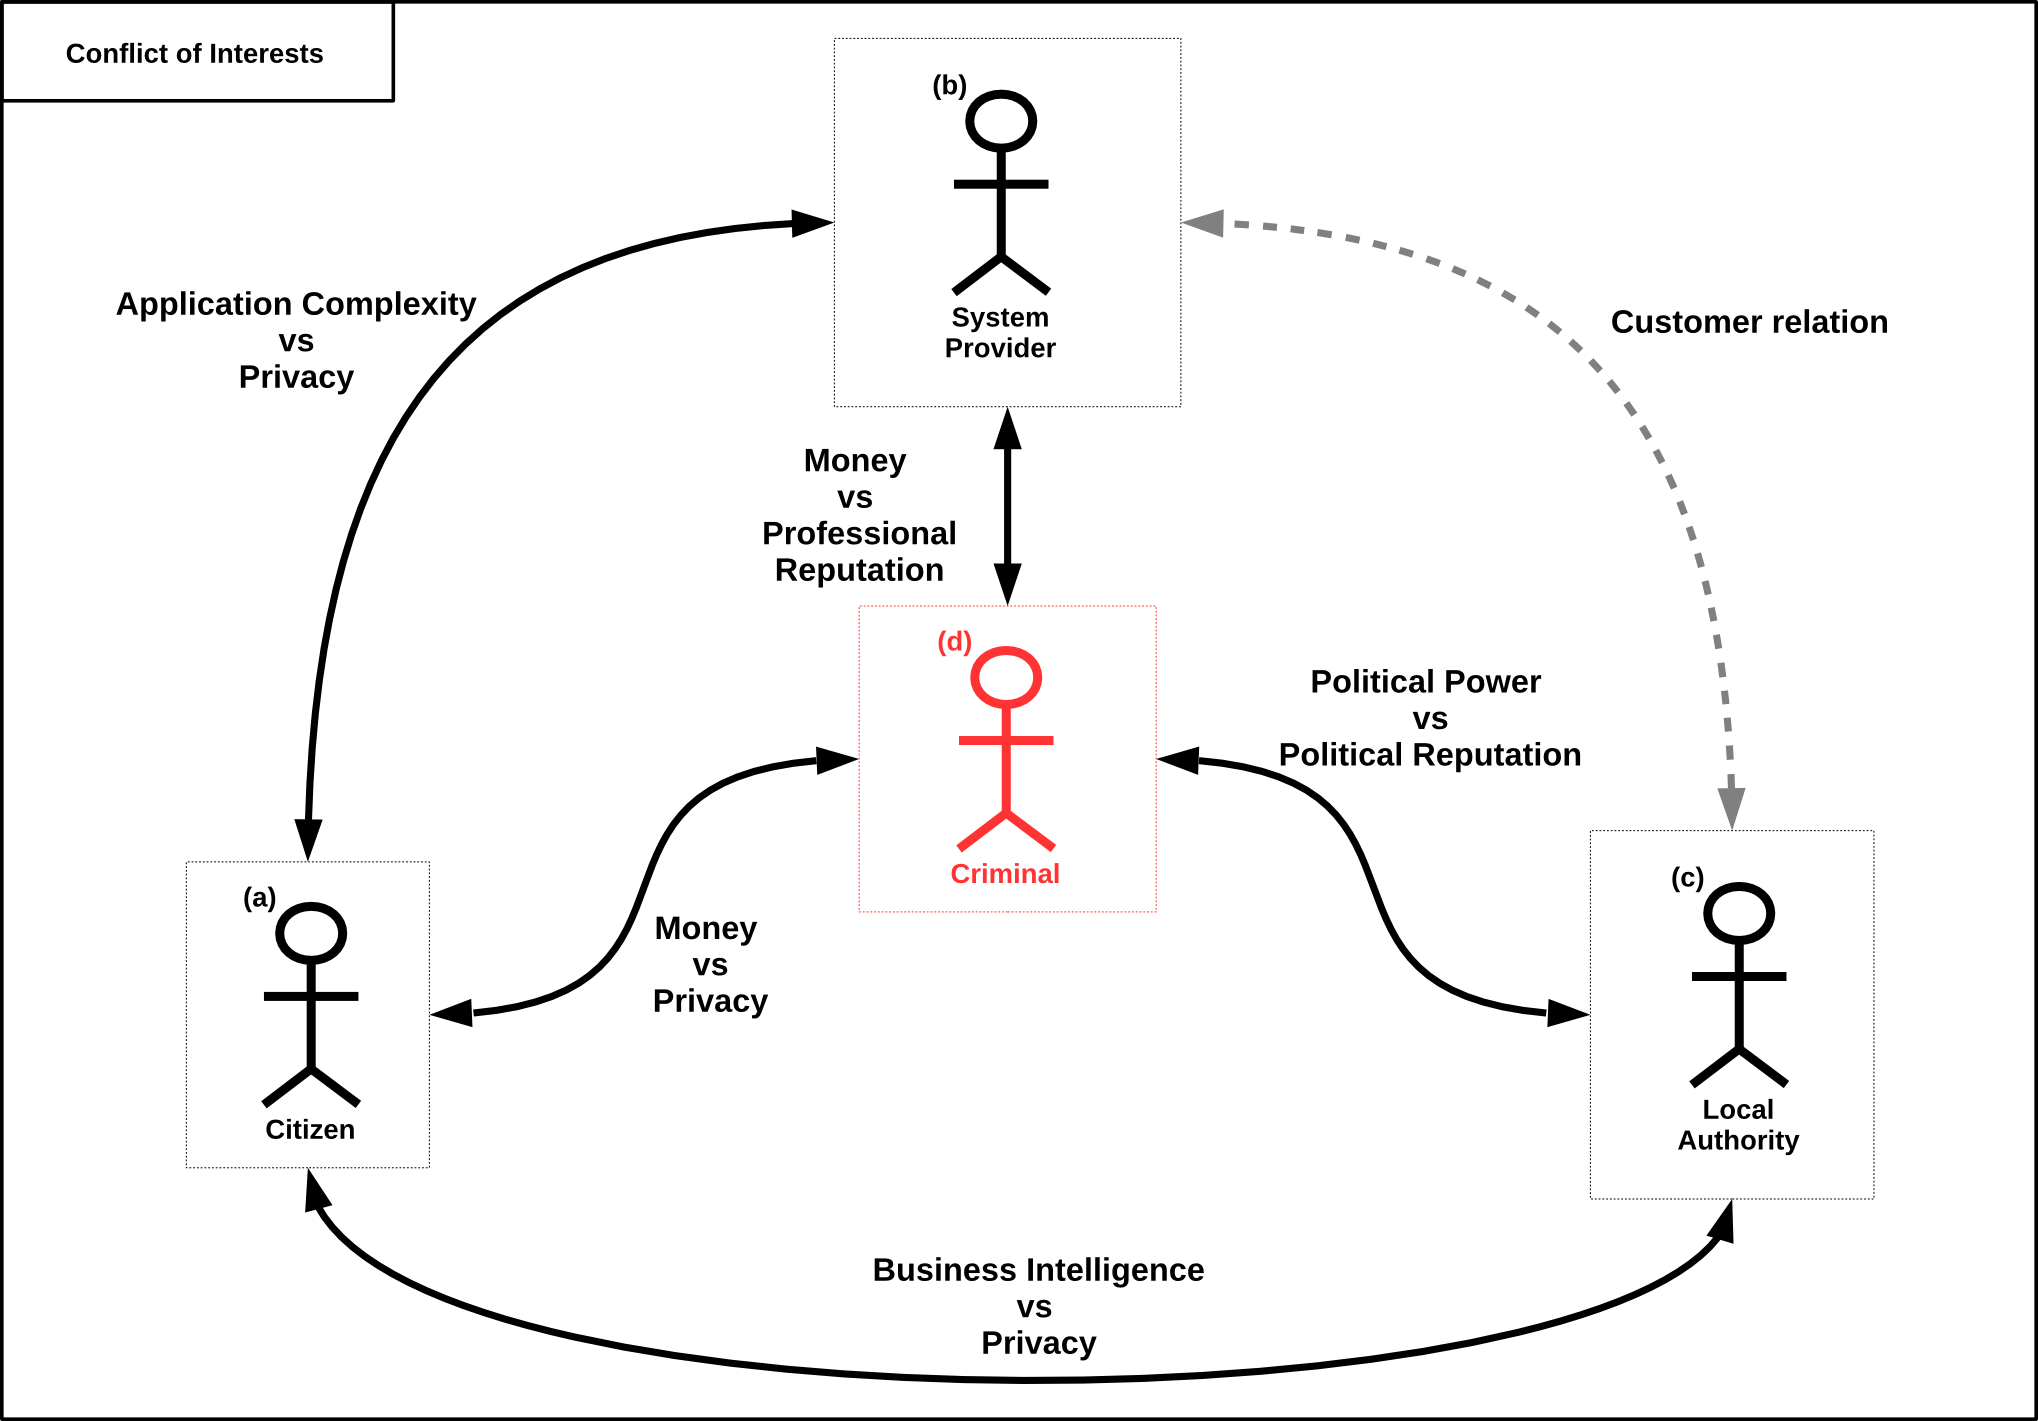
\includegraphics[width=\textwidth]{diagrams/png/conflict-of-interests.png}
\caption{Live+Gov Conflicts of Interests}
\label{figure:Live+Gov Conflicts of Interests}
\end{figure}

%TODO: Adapt Figure


\textbf{System Complexity vs Privacy.}
System Providers offer a service to Local Authorities, which is to provide and maintain a monitoring and mining system, e.g. for public mobility.
This system shall produce business intelligence, so that Local Authorities can improve their public services.
This task in it self has a high technical complexity and is the sole asset with financial return for System Providers.
However, this task operates on privacy sensitive data provided by monitored Citizens.
In order to ensure their privacy, System Provider would have to implement additional mechanisms, which allow Citizens to exercise control of their data.
This will not only raise the complexity of the monitoring and mining system, System Providers also have to layout the complexity in a comprehensible manner.
To effectively enable Citizens to preserve their privacy, they need to know what happens with their data.

\textbf{Business Intelligence vs Privacy.}
Local authorities order a monitoring and mining system from system providers, which allows them to produce business intelligence for public services.
The system is an investment for local authorities, so they are interested in as much intelligence as possible to achieve a profitable return.

The gained intelligence is the result of data mining conducted on privacy sensitive data of participating citizens.
They are interested in the successful usage of their data, in a sense that they are also benefactors, e.g. improvement of public mobility.
The main interest of citizens lies in maintaining control over their data and protecting their rights to privacy.
In order do that, they need full disclosure of the processing steps and the purposes their data is used for, and to be given a choice whether such processing should be allowed for their own data.

\textbf{Power of External vs. Privacy.}
Externals which are in a social relation to the citizen can have an interest in obtaining further information in order to gain power.
In the most simplistic example this could be a man wanting monitor the activities of his spouse.
Another example is a Government spying on it's citizens in order to suppress opposition.
An additional twist in the last example is, that there can be legal regulations that require the service provider to support the Governments invasion of the citizens privacy.

\textbf{Financial Profit of External vs Privacy.}
Externals can gain financial profit from stealing privacy sensitive data.
For example by selling raw contact information to advertisers or by selling mined data to insurance companies, or intermediaries like scoring companies.
In such cases, citizens lose complete control over their data.

\textbf{Financial Profit of External vs Reputation of System Providers.}
Externals have various business models as optional foundation for attacks on System Providers.
For instance, they can try to invade the infrastructure for e-espionage reasons, to get control over servers to create a bot-net or to steal user data.
All these approaches are motivated by financial interests.
Gathered information can be sold, zombie servers can be leased.

A successful attack proves the technical competence of system providers wrong and subsequently harms their professional reputation.
This can lead to a loss of future customers or a decrease of stock price for registered companies.
Eventually also the financial interests of system providers are endangered.

\textbf{Political Activism vs Reputation of Local Authority.}
Besides monetary reasons, externals can be motivated by political reasons to attack the monitoring and mining system.
Externals can break the system to make a political statement of their own,
or they can steal user data to prove the system insecure.
Both would harm the reputation of local authorities, who endangered the privacy of the citizens.


\subsubsection{Vulnerabilities}
\label{subsubsection:Vulnerabilities}
This section outlines the vulnerabilities (Figure \ref{figure:Live+Gov Vulnerabilities}) of the proposed monitoring and mining system.
Note that vulnerabilities are not necessarily of technical nature.
The weaknesses of IT systems are often created due to misuse or misconfiguration of the various components by one or more actors.

\begin{figure}
\centering
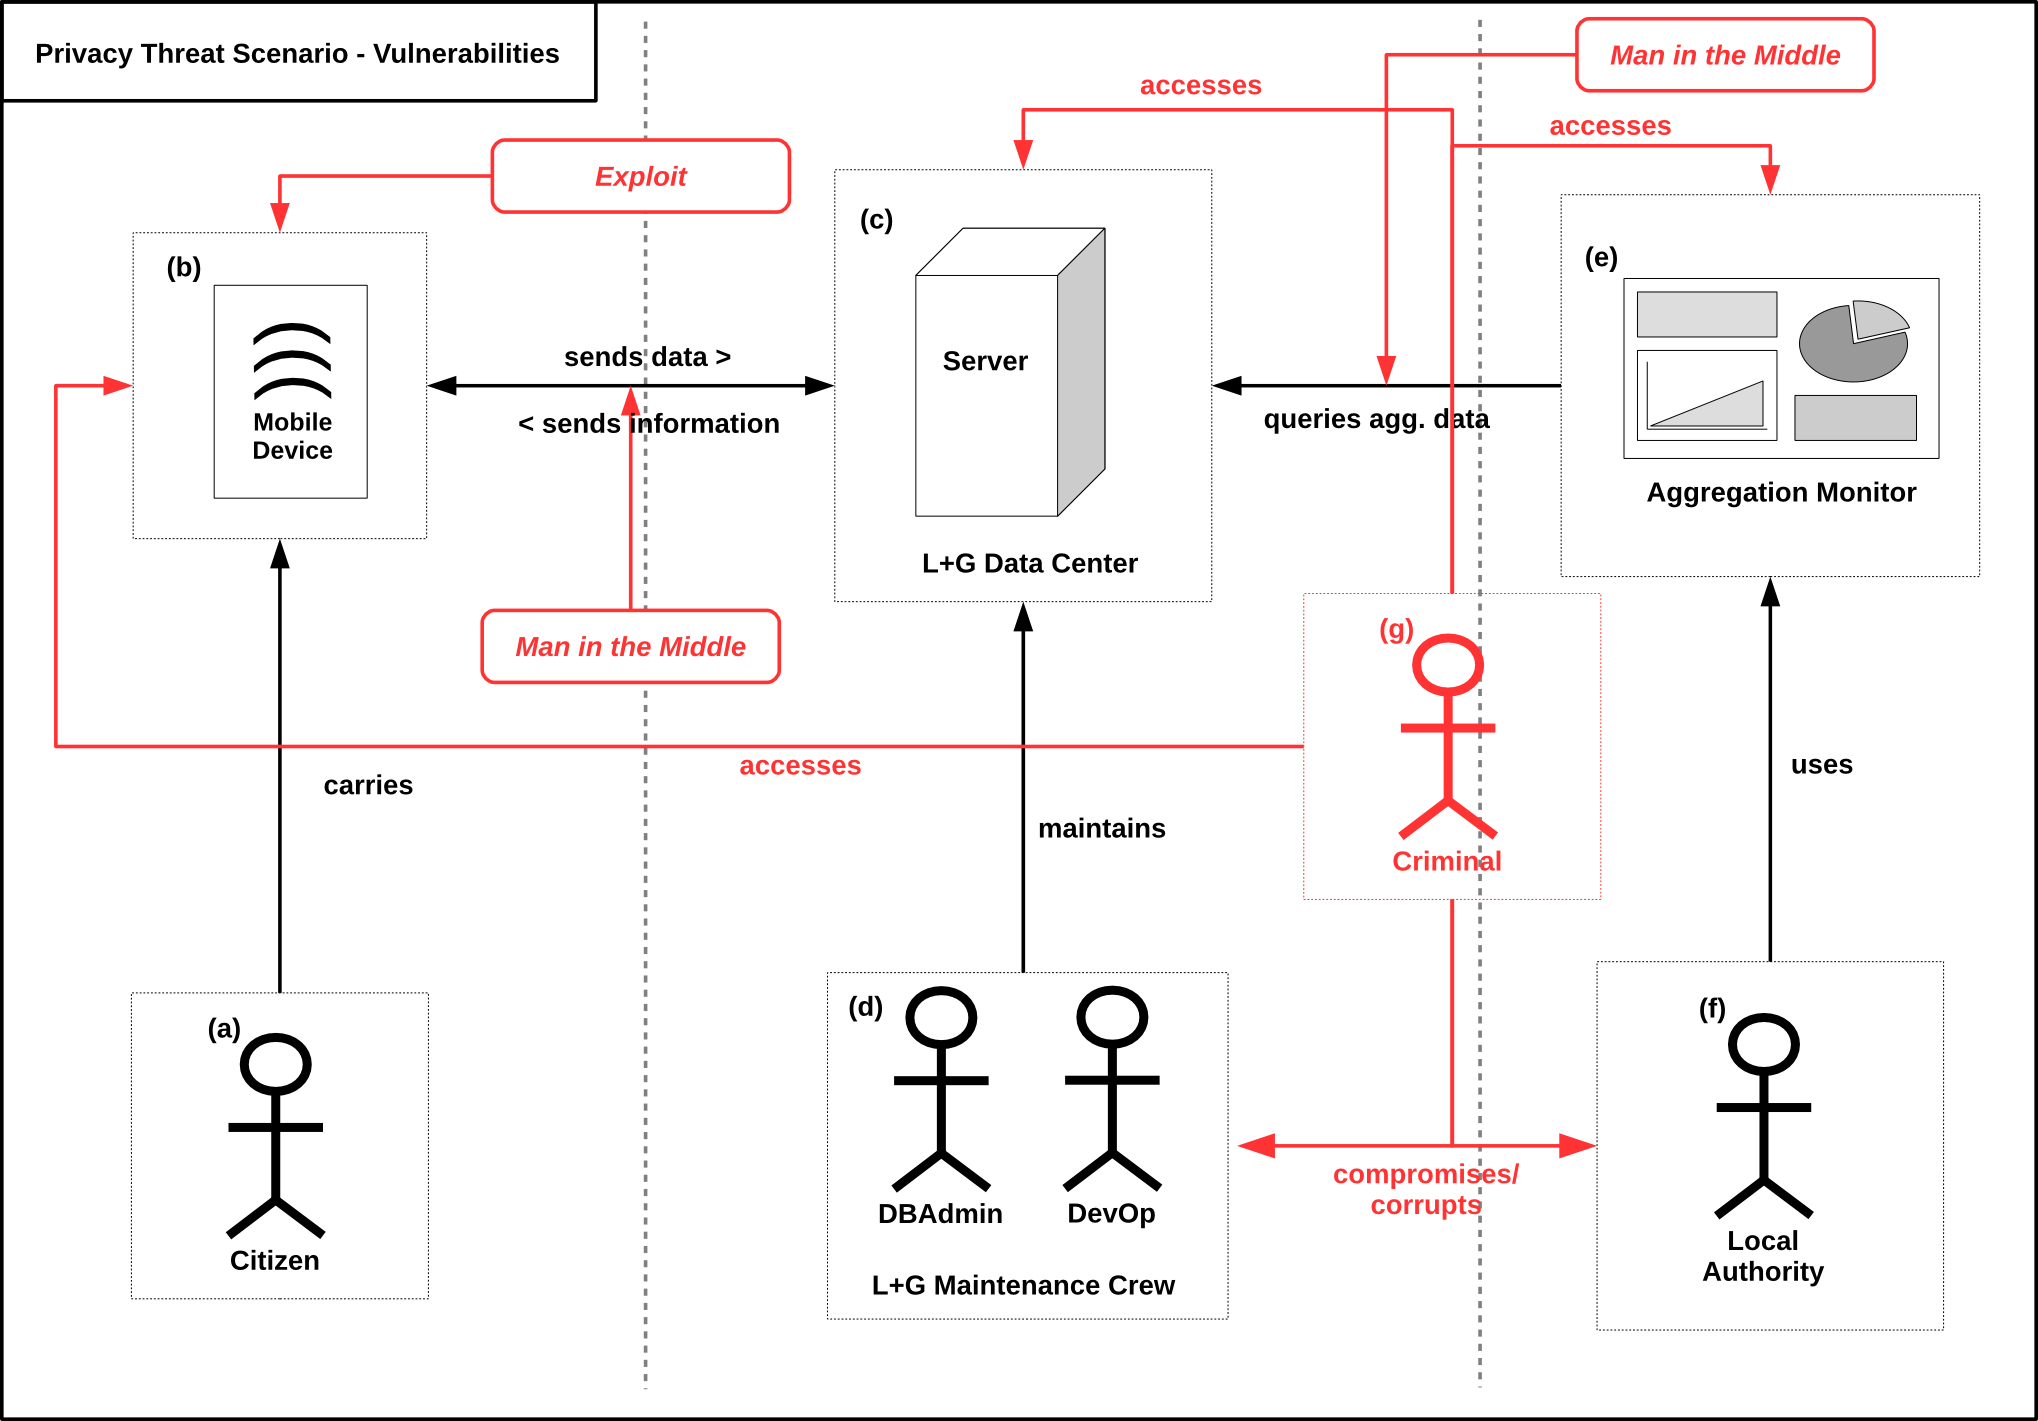
\includegraphics{diagrams/png/scenario-vulnerabilities.png}

\begin{flushleft}
\scriptsize
\textbf{Legend:}

\begin{itemize}
\itemsep1pt\parskip0pt\parsep0pt
\item
  \textbf{(a) Citizen:} User of the L+G client application whose privacy
  is at stake.
\item
  \textbf{(b) Mobile Device:} Runs the L+G client application, produces
  and stores data sensitive to the users privacy.
\item
  \textbf{(c) L+G Data Center:} Runs the L+G services, proccesses and
  stores user data.
\item
  \textbf{(d) L+G Maintenance Crew:} Technical staff with access to
  critical infrastructure.
\item
  \textbf{(e) Aggregation Monitor:} Interface to aggregated user data.
\item
  \textbf{(f) Local Authority:} Provider of the L+G system.
\item
  \textbf{(g) Criminal:} Threatens the L+G system and Citizen privacy.
\end{itemize}
\end{flushleft}

\caption{Live+Gov Vulnerabilities}
\label{figure:Live+Gov Vulnerabilities}
\end{figure}


\textbf{Insecure Infrastructure.}
The proposed monitoring system consists of many hardware and software components, each with its own concrete weaknesses.
For instance, operating systems can be outdated or not subject to frequent updates or virus scans.
Web-applications can be carelessly implemented and not protected against SQL-Injections or Cross-Site-Scripting attacks.
Databases can be ill-configured, so that access from outside the system is possible.
All those weak points can be subject to various known exploit techniques.


\textbf{Insecure Data Transmission.}
The proposed monitoring and mining system uses HTTP to exchange data between the Sensor Collector, the Data Center and the Report Tool.
Per default, HTTP is a clear text protocol.
This means, one can intercept the connection and read all sensitive information, which is send between the components.
That is: passwords, raw sensor data and data mining results

\textbf{Unhappy Employees.} Susceptible for social engineering.
%TODO: Add description

\textbf{Inadequate Access Rules.}
The proposed IT system infrastructure has various accesses to privacy sensitive data.
System Provider staff has access to Data Center hardware and software like databases, web-servers and other inspection tools.
Local Authority staff has access to the Report Tool.
This all enables staff members to have potential access to privacy sensitive information.
Those accesses have to be secured against unauthorized third parties.
Moreover, we need to ensure that no single person has to many access rights.
For example, a system administrator should not be able to secretly download the whole database on a flash-drive.

\textbf{Unaware Monitoring Subjects.}
We define privacy as one's ability to control information about oneself. 
In order to do that, monitored subjects need to know, that they are monitored, who monitors them, what information is recorded and for what purposes.
Subjects who are not aware of these things cannot effectively preserve control and thus lose their privacy.

%TODO
- No Privacy Policy
- No Information about Processing, Access rules, 3rd party disclosure


\subsection{Step 2. Potential Analysis}

\subsubsection{Threats}
This section outlines the potential threats (Figure \ref{figure:Live+Gov Threats}) for Citizen privacy in the proposed monitoring and mining System.
We derive threats from known conflicts of interests \ref{subsubsection:Conflicts of Interests} and vulnerabilities \ref{subsubsection:Vulnerabilities}

\subsection{Step 2. Potential Analysis}

\subsubsection{Threat Specification}

\textbf{Man In The Middle:}
Lorem ipsum dolor suit amet, ...

\textbf{Exploit:}
Lorem ipsum dolor suit amet, ...

\textbf{Corruption:}
Lorem ipsum dolor suit amet, ...

\textbf{Intrasparency:}
Lorem ipsum dolor suit amet, ...


\begin{figure}
\centering
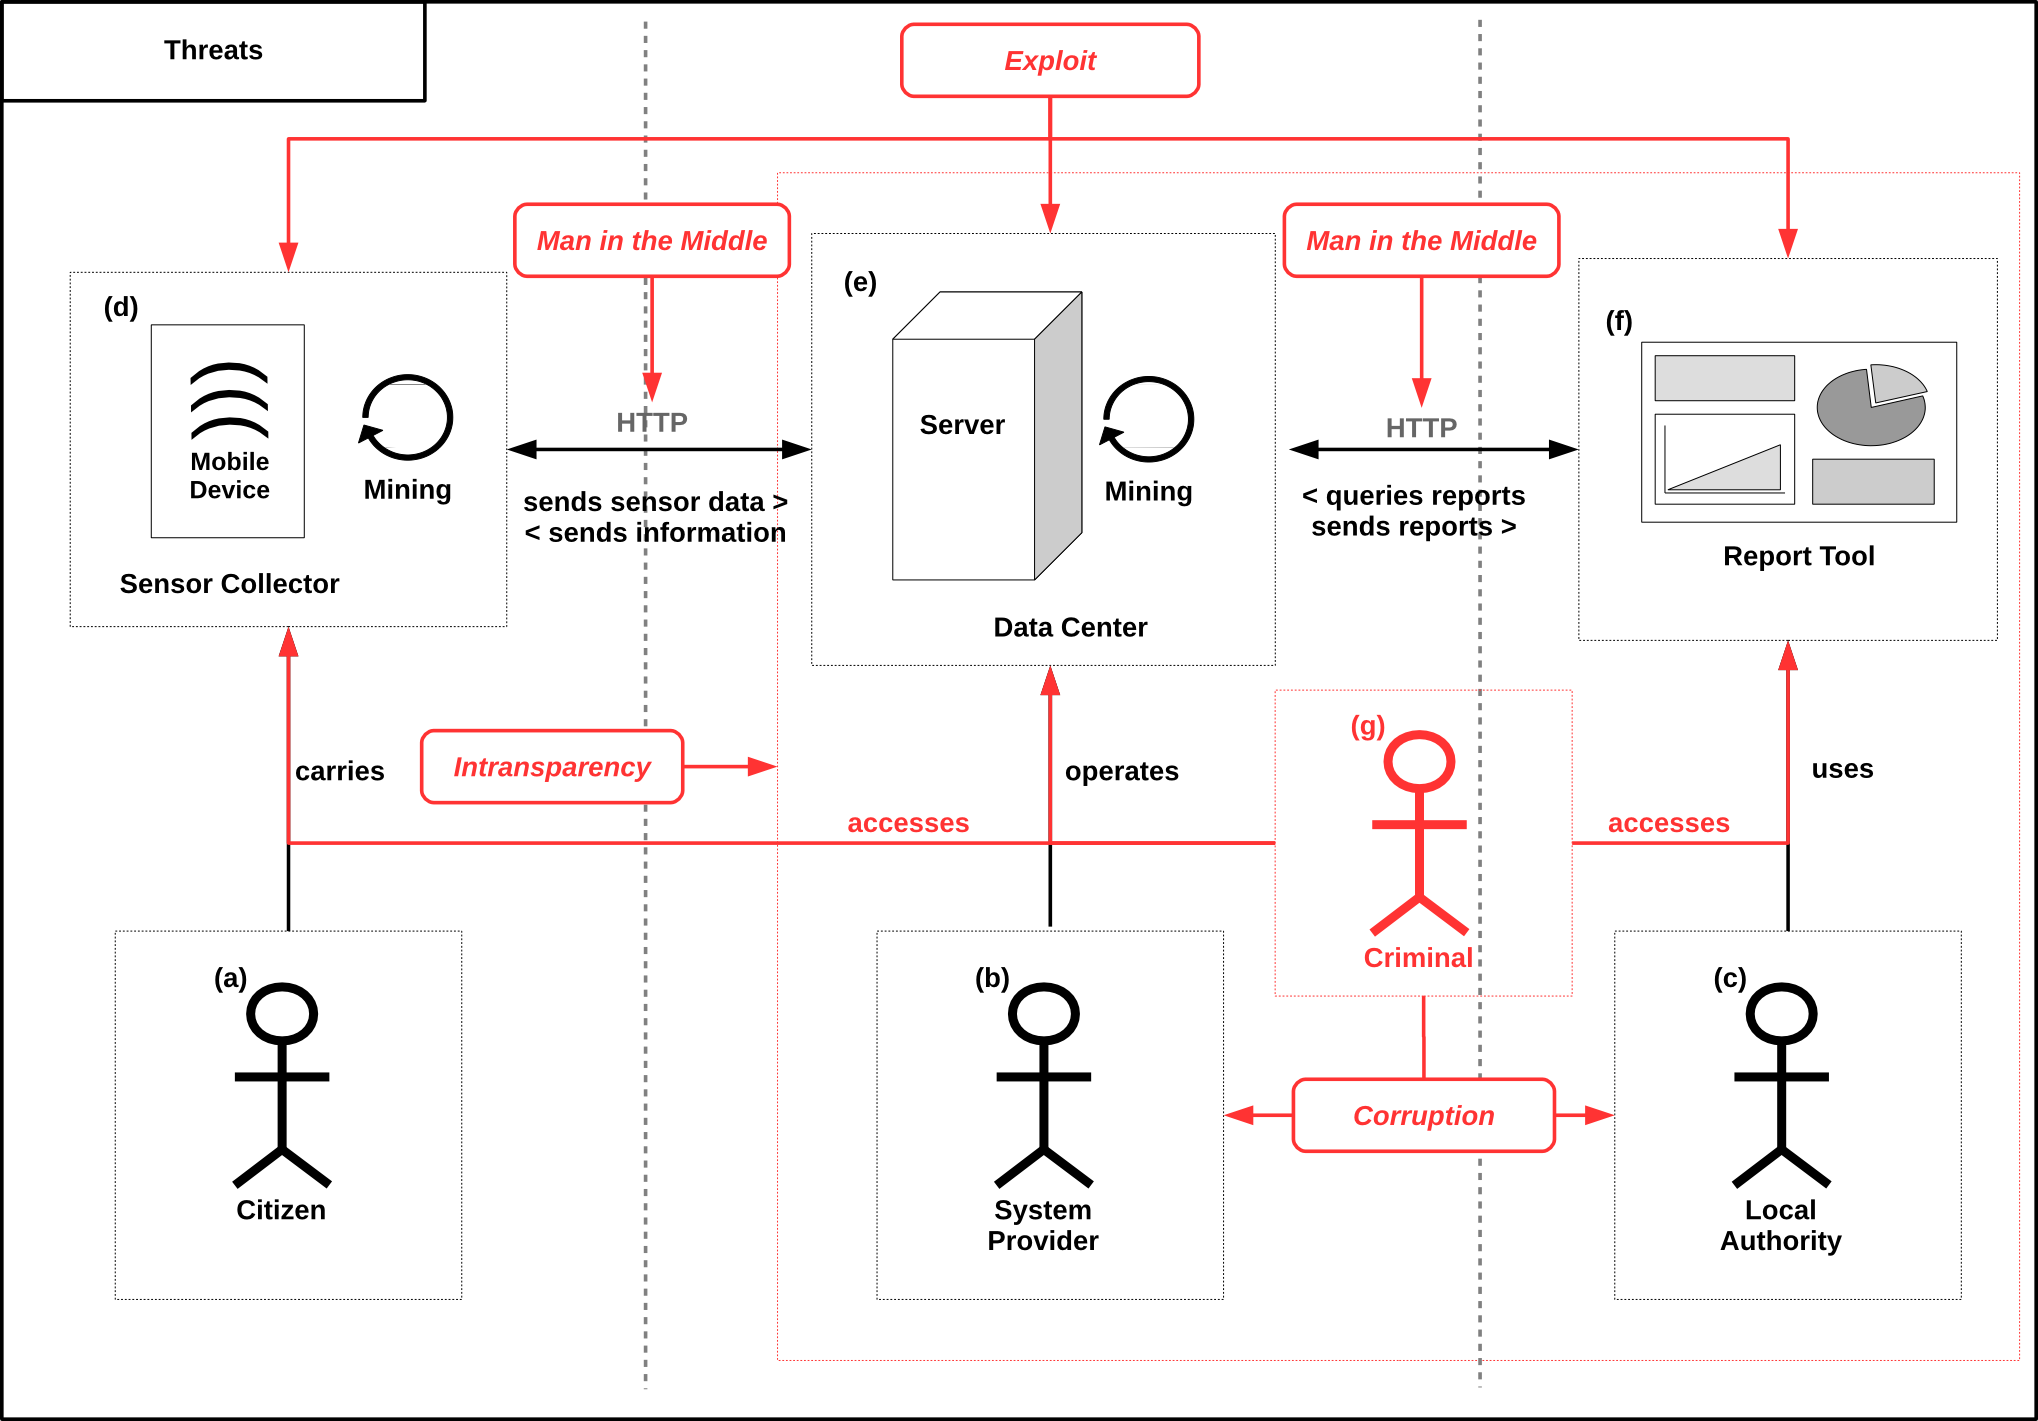
\includegraphics[width=\textwidth]{diagrams/png/threats.png}

%\begin{flushleft}
%\scriptsize
%\textbf{Legend:}
%
%\begin{itemize}
%\itemsep1pt\parskip0pt\parsep0pt
%\item
%  \textbf{(a) Citizen:} User of the L+G client application whose privacy
%  is at stake.
%\item
%  \textbf{(b) Mobile Device:} Runs the L+G client application, produces
%  and stores data sensitive to the users privacy.
%\item
%  \textbf{(c) L+G Data Center:} Runs the L+G services, proccesses and
%  stores user data.
%\item
%  \textbf{(d) L+G Maintenance Crew:} Technical staff with access to
%  critical infrastructure.
%\item
%  \textbf{(e) Aggregation Monitor:} Interface to aggregated user data.
%\item
%  \textbf{(f) Local Authority:} Provider of the L+G system.
%\item
%  \textbf{(g) Criminal:} Threatens the L+G system and Citizen privacy.
%\end{itemize}
%\end{flushleft}

\caption{Live+Gov Threats}
\label{figure:Live+Gov Threats}
\end{figure}

\begin{figure}
\centering
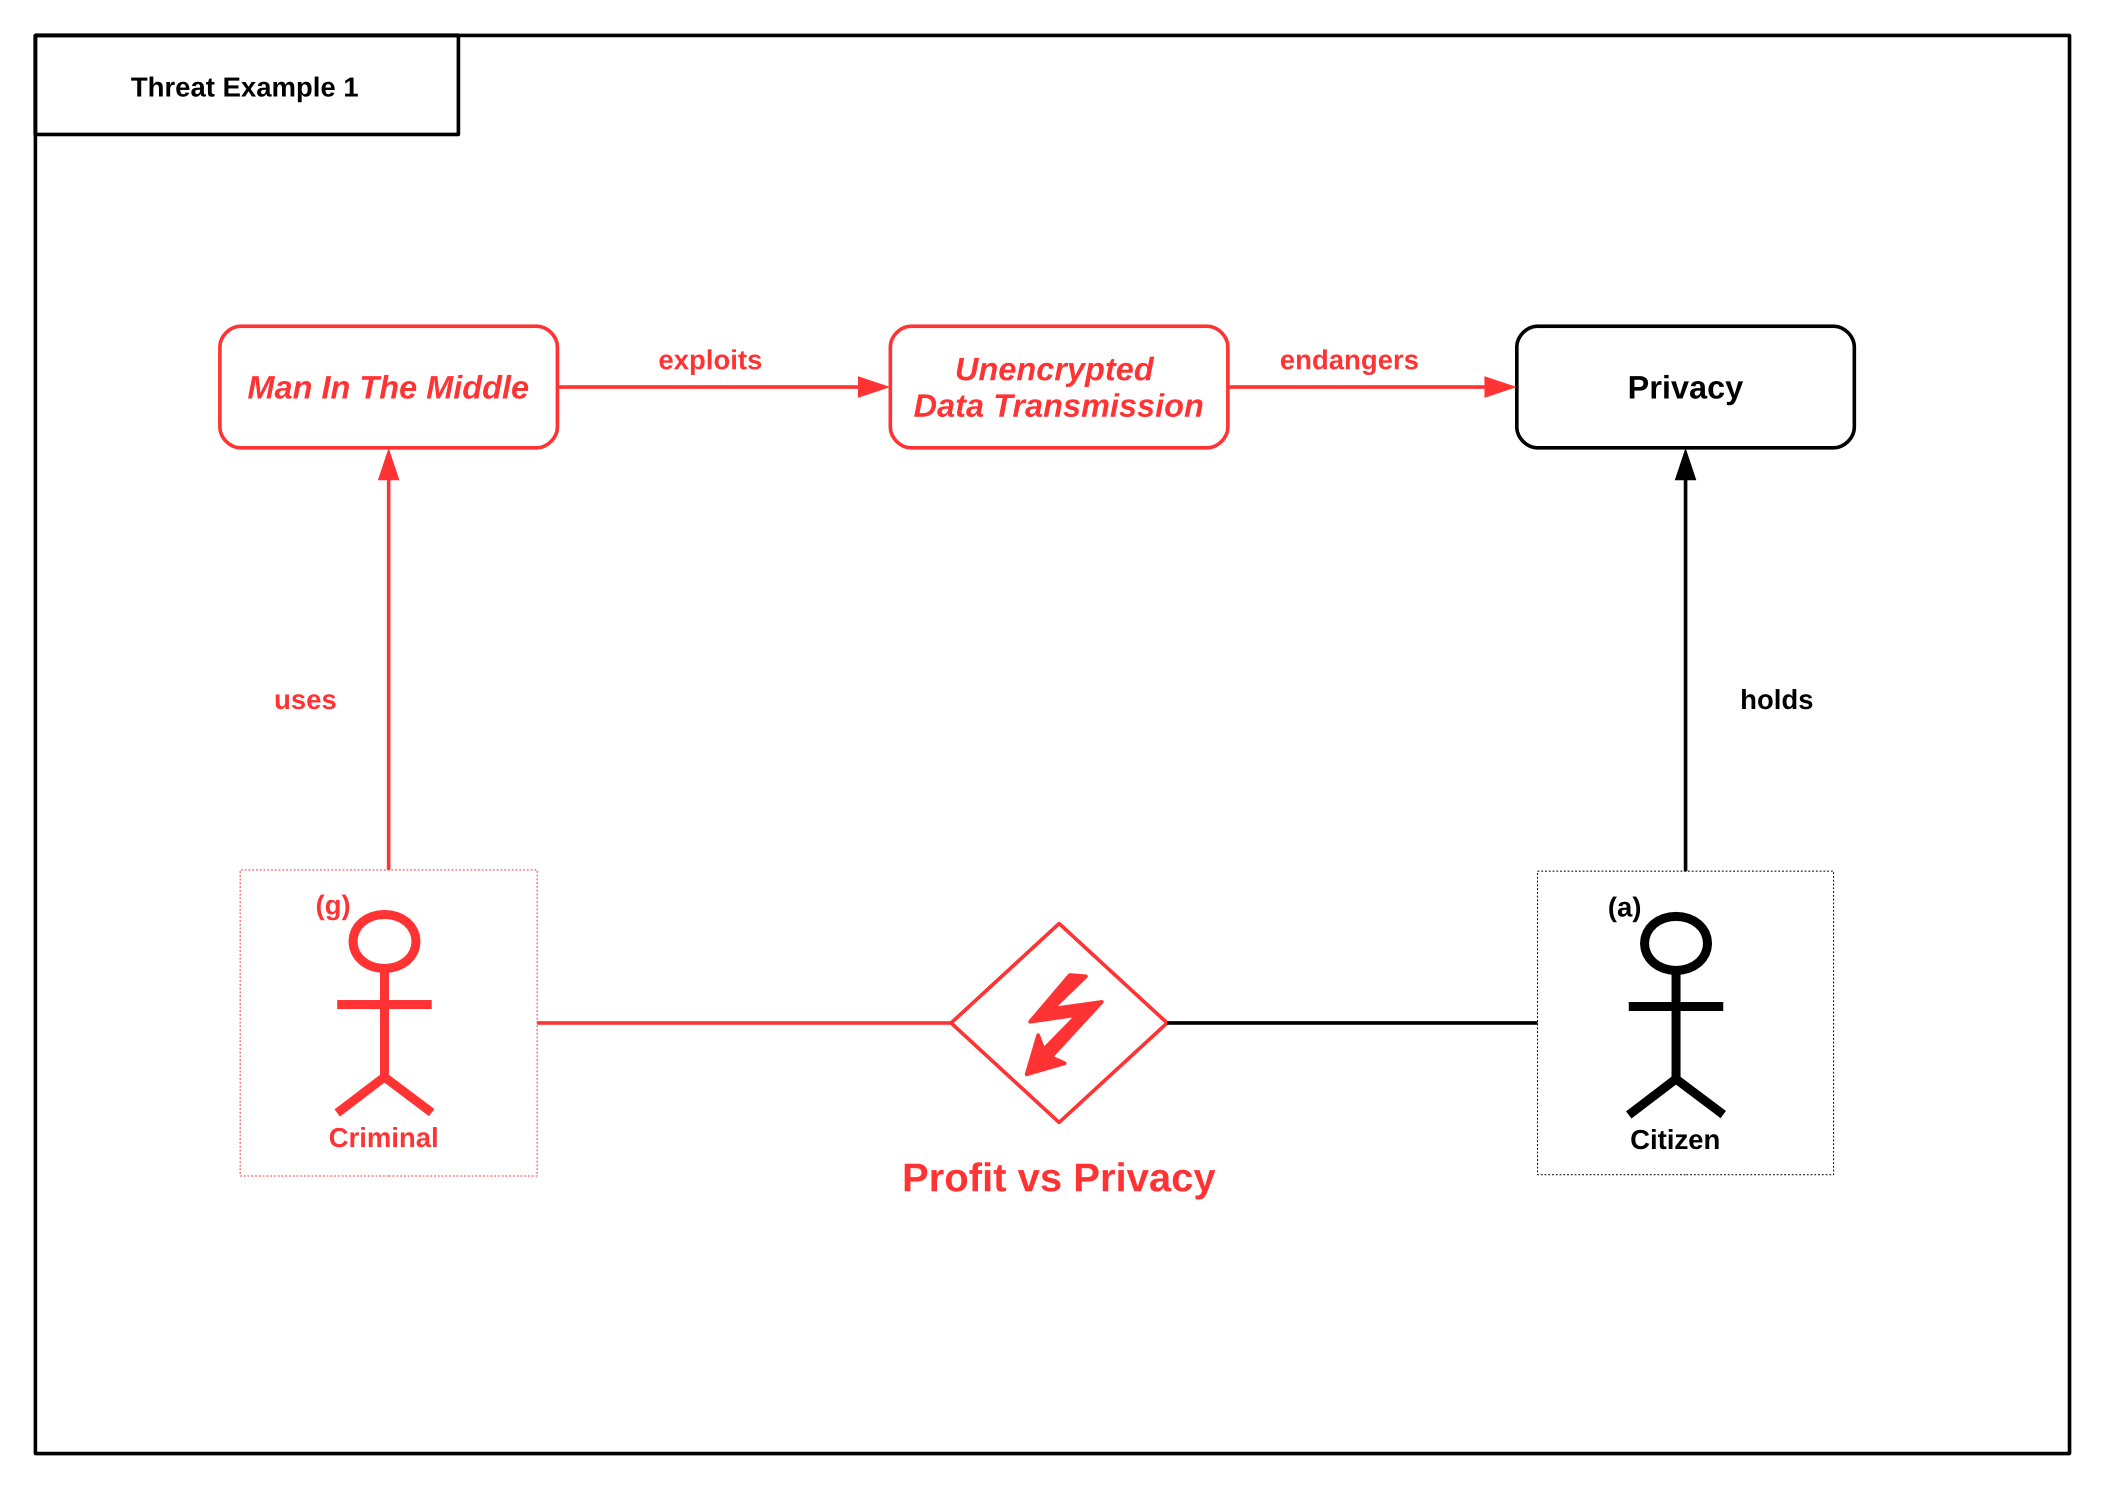
\includegraphics[width=\textwidth]{diagrams/png/man-in-the-middle.png}


\caption{Threat Example 1: Man In The Middle}
\label{figure:Threat Example 1: Man In The Middle}
\end{figure}

\begin{figure}
\centering
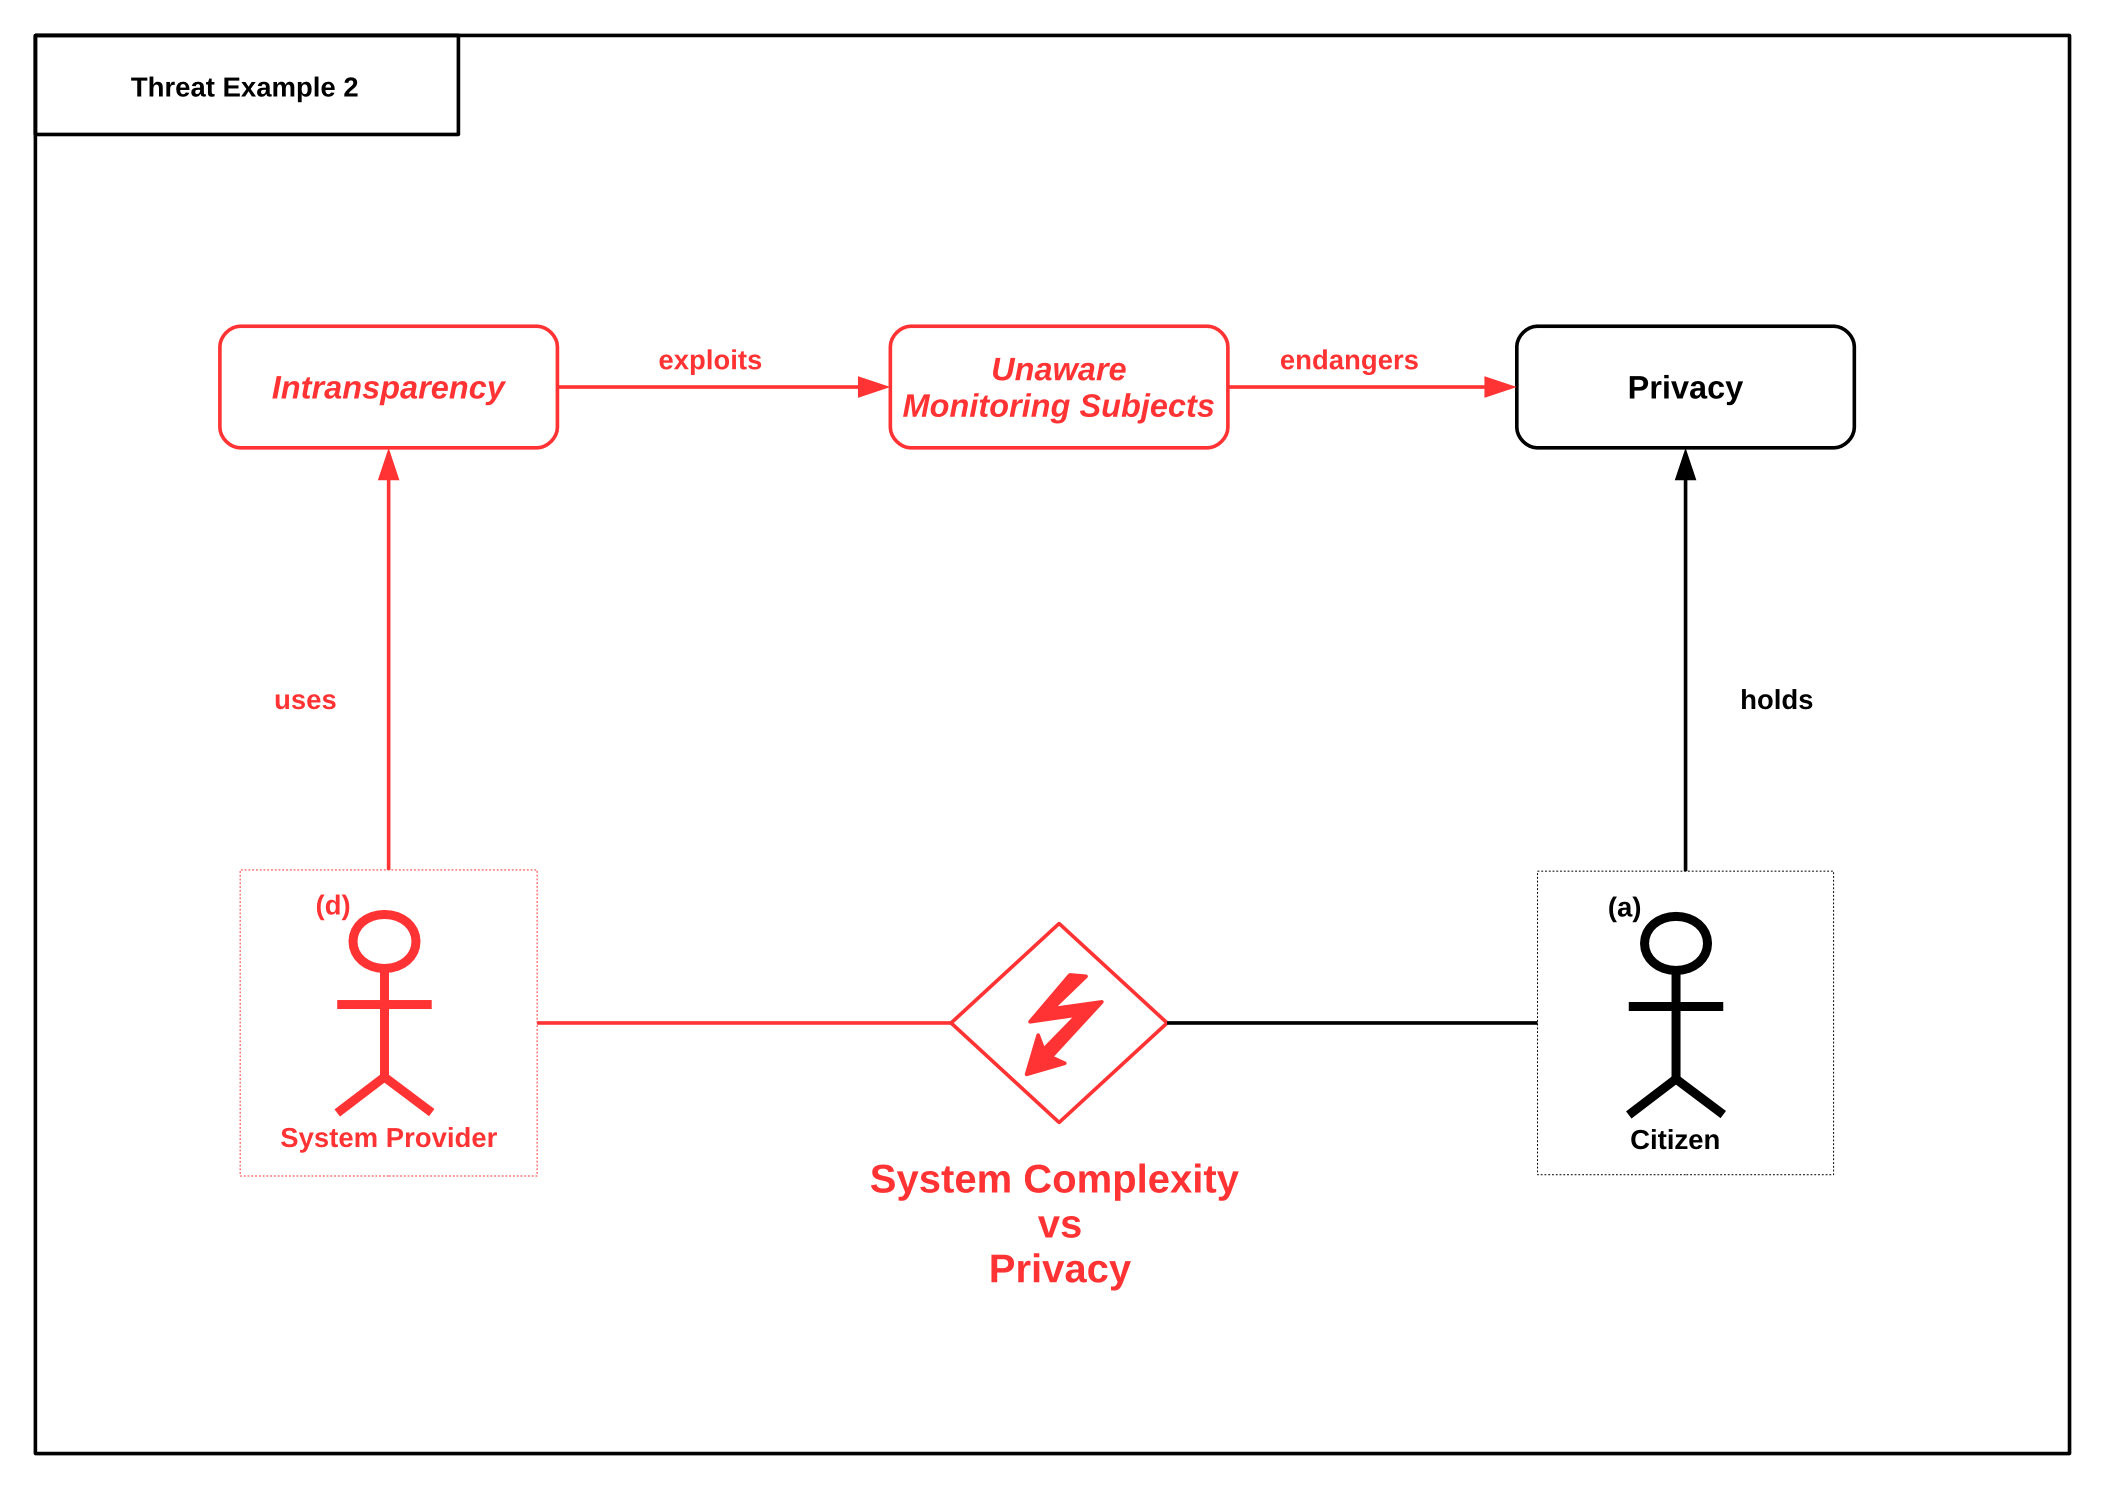
\includegraphics[width=\textwidth]{diagrams/png/intransparency.png}


\caption{Threat Example 2: Intransparency}
\label{figure:Threat Example 2: Intransparency}
\end{figure}

% =================================================
% Threat Table Macros

% Const Column Width
\newcommand{\ThreatTableColWidth}{5cm}

% Const Header Row Height
\newcommand{\ThreatTableHeaderRowHeight}{0.5cm}

% Const Content Row Height
\newcommand{\ThreatTableContentRowHeight}{1cm}

% Define Header Cell Makro
\newcommand{\ThreatTableHeaderCell}[1]{
\begin{minipage}[t][\ThreatTableHeaderRowHeight][c]{\ThreatTableColWidth}
\centering
\scriptsize
\textbf{#1}
\end{minipage}
}

% Define Content Cell Makro
\newcommand{\ThreatTableContentCell}[1]{
\begin{minipage}[t][][c]{\ThreatTableColWidth}
\begin{flushleft}
\tiny
#1
\newline
\end{flushleft}
\end{minipage}
}

% Define Header Row Makro
\newcommand{\ThreatTableHeaderRow}[4]{
\ThreatTableHeaderCell{#1}
&\ThreatTableHeaderCell{#2}
&\ThreatTableHeaderCell{#3}
&\ThreatTableHeaderCell{#4}
\\ \hline
}

% Define Content Row Makro
\newcommand{\ThreatTableContentRow}[4]{
\ThreatTableContentCell{#1}
&\ThreatTableContentCell{#2}
&\ThreatTableContentCell{#3}
&\ThreatTableContentCell{#4}
\\ \hline
}

%  Define Threat Table Environment
\newenvironment{ThreatTable}
{
\begin{tabular}{|c|c|c|c|}
\hline
\ThreatTableHeaderRow
{Description}
{Conflict of Interest}
{Vulnerabilites}
{Assets (Privacy Types)}
}
{\end{tabular}}


% =================================================
% Threat Table Content

\begin{landscape}
\begin{figure}
\centering
\begin{ThreatTable}

\ThreatTableContentRow
{\textbf{(Zero Day) Exploits}
\\A criminal uses (Zero Day) Exploits to obtain access to hardware or software which stores or processes
privacy sensitive data in order to get that data.}
{Criminals want to obtain access or data for personal profit, i.e. by (re-)selling the data or  by processing it themselves. 
However, criminals may have no financial interest, they could also gain personal (ego) profit by testing proof-of-concept attacks.
\\\textbf{Criminal vs Citizen}
\\Citizens only allowed Local Authorities to use their data. They want their data to be secret to others. (Additionally, citizens are
also interested in a working system, which they payed for via taxes.)
\\\textbf{Criminal vs Local Authorities}
\\Local Authorities have capital and reputation invested in a working system. Successful attacks undermine both.
\\\textbf{Criminal vs Maintenance Staff}
\\Staff members have a professional ethos and a duty to provide working systems. Successful attacks offend the former and obstruct the latter.
\\Staff member employed by L+G or contractor. The Business operation is thretened by loss of confidential data.
}
{Unsecured Hardware- or Software-Interfaces}
{\textbf{Explicit:} 1,4,6,7}

\ThreatTableContentRow
{\textbf{Man in the Middle} 
\\A criminal intercepts communication between mobile device and server or between server and application.}
{\textit{Like Exploits}}
{Unencrypted hardware or software communication}
{\textbf{Explicit:} 1,4,6,7}

\ThreatTableContentRow
{\textbf{Corrupt Employees} 
\\ An employee abuses his database access to obtain private citizen data in order to sell it to advertisers.}
{\textbf{(Corrupt) Employee vs Citizen} 
\\ Corrupt Employees want to make personal profit by selling citizen data. 
Citizens provide data for public improvement, they don't want their data to be used for other purposes, which
may lead to negative effects for themselves.
Employees in general need easy database access to do their job. But this also means easy access to privacy
sensitive data of citizens. This diametrically opposes the interest of citizens to have such information unknown
to other individuals.}
{Full database access of Employees}
{\textbf{Explicit:} 1,4,6,7}

\ThreatTableContentRow
{\textbf{Corrupt Local Authorities}
\\A member of the Local Authority abuses his access to applications 
to obtain aggregated citizen data in order to use it for illegitimate purposes, e.g. selling it.}
{\textbf{(Corrupt) Local Authority Member vs Citizen}
\\\textit{Like Corrupt Employees}}
{Full application access of Local Authorities}
{\textbf{Explicit:} 1,4,6,7}

\ThreatTableContentRow
{\textbf{Careless Citizen}
\\A careless citizen allows others (Criminals) to have unrestricted access to his mobile device. 
Hence, he creates to possibility to install spy-ware or have the device destroyed.}
{\textbf{Criminal vs Citizen}
\\Criminals want to have access to mobile devices to obtain private data of citizens in order to 
gain personal profit - or to simply render the device useless. On the other hand, citizens have a 
natural interest in keeping personal data secret in order to prevent financial loss or because having
sensitive information accessible to others violates their privacy.}
{Insufficient access rules for mobile devices}
{\textbf{Explicit:} 1,4,6,7}

\ThreatTableContentRow
{\textbf{Intransparent Data Mining}
\\Local Authorities or System Providers use their technical knowledge, data mining capabilities and 
additional data sources to obtain/create more information about citizens.}
{\textbf{Citizen vs Local Authority or System Provider}
\\Citizens only agreed to share certain sensitive data with Local Authorities and System Providers to help society.
They are not interested in negative effects as a result of such a good willing act.
However, Local Authorities and System Providers have an interest to maximize the profit of their investments.
Local Authorities could (secretly) use mined data for security or health care issues. System Providers could
(secretly) sell mined data to illegitimate customers, e.g. the SCHUFA. This could lead to repressive behaviour of law
enforcement or negative scores.}
{Unaware Citizens}
{1,2,3,4,5,6,7}

\end{ThreatTable}

{\scriptsize (\textbf{Note for Meeting:} I think we need discrete (numbered) lists of interests for each actor in the \textit{Humans} section.)}

\caption{Threat Table}
\end{figure}
\end{landscape}


\subsubsection{Threat Risk Evaluation}

% Todo: use sensor privacy matrix and implicit sensor privacy matrix for threat risk evaluation

\textbf{Sensor Privacy Matrix}

%\includegraphics{../diagrams/png/sensor-privacy-matrix.png}
\begin{figure}
\centering
\includegraphics[width=\textwidth]{diagrams/png/sensor-privacy-matrix.png}


\begin{flushleft}
\scriptsize
\textbf{Legend:}
\begin{itemize}
\itemsep1pt\parskip0pt\parsep0pt
\item
  The x-axis lists the 7 Types of Privacy according to Friedewald et al.
\item
  The y-axis lists all mobile sensors currently used by the Live+Gov
  procject.
\item
  The big black bullet point dentotes that there is a \textbf{direct}
  violoation of a privacy type from a sensor
\end{itemize}
\end{flushleft}

\caption{Live+Gov Sensor-Privacy Matrix}
\label{figure:Live+Gov Sensor-Privacy Matrix}
\end{figure}

%\begin{figure}
\centering
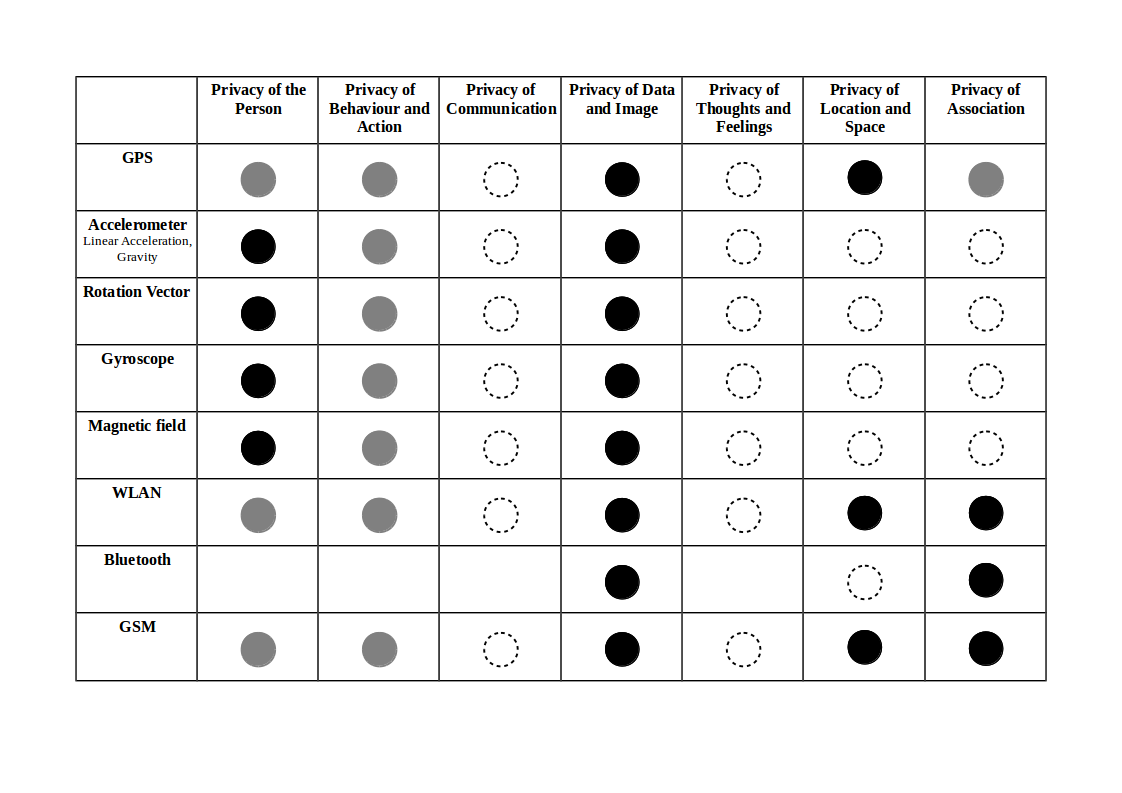
\includegraphics[width=\textwidth]{diagrams/png/implicit-sensor-privacy-matrix.png}


%\begin{flushleft}
%\scriptsize
%\textbf{Legend:}
%\begin{itemize}
%\itemsep1pt\parskip0pt\parsep0pt
%\item
%  The x-axis lists the 7 Types of Privacy according to Friedewald et al.
%\item
%  The y-axis lists all mobile sensors currently used by the Live+Gov
%  procject.
%\item
%  The big black bullet point dentotes that there is a \textbf{direct}
%  violoation of a privacy type from a sensor
%\end{itemize}
%\end{flushleft}

\caption{Live+Gov Implicit Sensor-Privacy Matrix}
\label{figure:Live+Gov Implicit Sensor-Privacy Matrix}
\end{figure}


\begin{itemize}

\item
\textbf{Privacy of The Person}

The \textbf{Privacy of The Person} is generally concerned with one could best understand as \emph{Biometric Privacy}. 
Friedewald et al. paraphrase it as \emph{``\om the right to keep body functions and body characteristics \om private''}. 
\textbf{Accelerometer}, \textbf{Rotation Vector} and \textbf{Gyroscope} measure the physical movement of the mobile device on all three axes. 
If the mobile device is carried \emph{``normally''} its safe to say that those sensors also measure the moments of its carrier. 
So his privacy is infringed regarding biometric behaviour, as it is captured automatically.
(\textbf{Note:} This is not to be confused with the \textbf{Privacy of Behaviour and Action} which is used for the social aspects of behaviour action, e.g.~praying, sexual habits or political activities.)

\item
\textbf{Privacy of Data and Image}

The \textbf{Privacy of Data and Image} demands, that \emph{``individual's data is not automatically available to other individuals''}. 
This type of privacy is trivially threatened because here sensor data is individual data, a priori. 
So every sensor violates the privacy of data and image, as data is transported into a foreign system where operators have access to it.


\item
\textbf{Privacy of Location and Space}

According to Friedewald et al., the \textbf{Privacy of Location and Space} is concerned with one's \emph{``right to move about in public or semi-public space without being identified, tracked or monitored.''}.
This is the location aspect of this type. The space aspect is concerned with one's \emph{``right to solitude''}, which generally includes one's right to an inviolate home and other private spaces. 
Obviously the \textbf{GPS} and \textbf{GSM} sensors violate such right about not being tracked, because they reveal the position of the mobile device and its carrier. 
The \textbf{GSM} sensor gives the exact cell, the mobile device has registered with at the current moment. 
The \textbf{GPS} sensor gives the current longitude and latitude, the current global position of the mobile device and its carrier, although there is some artificial inaccuracy within civil use.

The \textbf{WLAN} and \textbf{Bluetooth} sensors record lists of the currently available local wireless networks and bluetooth clients. 
If such are known stationary entities, those sensors are considered as dangerous as the \textbf{GSM} sensor for the carriers locational privacy.

The \textbf{Magnetic field} sensor is not regarded very dangerous to the carrier's privacy, because it does not allow very precise localization.
But it can limit the possibilities for the global position of the mobile device. 
Here, it is just named for completeness sake.

\item
\textbf{Privacy of Associtation}

The \textbf{Privacy of Association} sates that everyone has the \emph{``right to associate with whomever they wish, without being monitored [automatically without reasonable suspicion]''}. 
This includes individuals and organizations. 
\textbf{WLAN} and \textbf{Bluetooth} sensors provide the ability to monitor such associations if their lists contain known entities. 
If one frequently connects with an organizational wireless network, e.g.~an university network, an association can be deduced (student or staff). The same goes for the \textbf{Bluetooth} sensor, if it is stationary. 
Additionally, if the recorded bluetooth clients are mobile, it is more or less possible to deduce association with the technical identity of (yet) anonymous individuals.

Additionally, the \textbf{GSM} sensor could provide the association with the GSM operator (\textbf{NEEDS TO BE VERIFIED!}).

\end{itemize}







\subsubsection{Security Requirement Specification}


\subsection{Step 3. Plan Development}

\subsection{Legal Privacy Requirements} \ref{sec:LEGAL_REQ}

\subsubsection{Security Measures}

\textbf{The 7 C's of user privacy control (Figure \ref{figure:The Seven Cs of User Privacy Control})}

This is a note on an excerpt from the article \emph{Sociotechnical
Architecture for Online Privacy} \cite{1} called
\textbf{The 7 C's of user privacy control}. Those 7 C's are aspects
which should be covered by measures for implementing user privacy. They
derive from an interpretation of privacy which could be summarized as
\emph{``One's ability to control/seclude information about oneself''}.

%\includegraphics{../diagrams/png/The7Cs.png}
\begin{figure}
\centering
\includegraphics[width=\textwidth]{diagrams/png/The7Cs.png}
\caption{The Seven Cs of User Privacy Control}
\label{figure:The Seven Cs of User Privacy Control}
\end{figure}


\begin{itemize}


\item
\textbf{Comprehension}

\emph{``Users should \textbf{understand} ho personal identifiable
information (PII) is handled, who's collecting it and for what purpose,
and who will process the PII and for what purpose. Users are entitled
to know all parties that can access their PII, the limits to processing
transparency, why the PII data is being requested, when the data will
expire (Either from a collection or database), and what happens to it
after that. This category also include legal rights around PII, and the
implications of a contract when one is formed.''}

This C implements transparency regarding user data and user privacy.
Comprehension should answer the following questions:

\begin{itemize}

\item
  \emph{WHO} collects data?
\item
  \emph{WHAT} data will be collected?
\item
  \emph{WHY} will data be collected and processed?
\item
  \emph{HOW} will data be collected and processed?
\item
  \emph{WHEN} will data expire?
\item
  What is allowed?
\item
  What choices ar possible?
\end{itemize}

All in all information of what's happening and why has to made
accessible for users.

\item
\textbf{Consciousness \textbf{(critical!)}}

\emph{``Users should \textbf{be aware} of when data collections occurs,
when a contract is being formed between a user and data collector when
their PII is set to expire, who's collecting the data, with whom the
data will be shared, how to subsequently access the PII, and the
purposes for which the data is being collected.''}

This C seems to be critical for privacy protection. Consciousness
complements Comprehension in respect that the latter just states that
hard facts need to be delivered. However, those facts might get hidden
in a terms and conditions section which nobody reads but still accepts
anyway. In order to prevent that Consciousness states that a certain
level of \textbf{Awareness} of those facts needs to be established.

\item
\textbf{Choice}

\emph{``Users should \textbf{have choices} regarding data collection
activities in terms of opting in or out, whether or not to provide data,
and how to correct their data.''}

Self explaining. This is the actual control enabled by the 7 C's.

\item
\textbf{Consent}

\emph{``Users must first \textbf{consent} (meaning informed, explicit,
unambiguous agreement) to data collection, use, and storage proposals
for any PII. Privacy consent mechanisms should explicitly incorporate
the mechanisms of comprehension, consciousness, limitations, and
choice.''}

This C might be special case of Choice. Before taking part a user should
have the choice whether to join or not (Opt-In).

\item
\textbf{Context}

\emph{``Users should \textbf{be able to change privacy preferences}
according to context. Situational or physical context - such as crowded
situations (for example, when at a service desk where several people
can listen in on your exchange when you provide a phone number, or when
you're in an online community chat room) - is different from when you
perform a buy transaction with Amazon.com or in rooms with cameras
(where digitization makes the information permanent and unmistakably
you) and data context (such as the sensitivity of data, for example
health data could dictate different actions on the same PII in different
contexts.''}

Self explaining. Refines Choice in context sensitive manner.

\item
\textbf{Confinement}

\emph{``Users should \textbf{be able to set limits} on who may access
their PII, for what purposes, and where and possibly when it may be
stored. Setting limits could provide some good opportunities for future
negotiation between vendors and users.''}

Self explaining. Refines Choice regarding data collection and
processing.

\item
\textbf{Consistency}

\emph{``Users should \textbf{anticipate} with reasonable certainty what
will occur if any action involving their PII is taken. That is, certain
actions should be predictable on user access of PII or giving out of
PII.''}

Information given by Comprehension needs to be reliable to found
choices.



\end{itemize}



\textbf{The 2 Steps of the 7 C's (Figure \ref{figure:The 2 Steps of the 7 Cs of User Privacy Control})}

If we look closer at the 7 C's and how they try to enable control, we
see that a 2 step approach is taken:

%\includegraphics{../diagrams/png/7Cs2Steps.png}
\begin{figure}
\centering
\includegraphics[width=\textwidth]{diagrams/png/7Cs2Steps.png}
\caption{The 2 Steps of the 7 Cs of User Privacy Control}
\label{figure:The 2 Steps of the 7 Cs of User Privacy Control}
\end{figure}


\begin{enumerate}

\item
\textbf{Enable \emph{Adequate} Control}

The 7 C's try to enable control through choices. A user should be able
to choose which data can be collected and processed depending on context
and who will have access to the data. But cannot be random. In order to
make substantiated choices and enable \emph{adequate} control a user
needs have

\begin{itemize}

\item
  \textbf{Comprehension:} access to hard facts
\item
  \textbf{Consistency:} trust that those facts are reliable
\item
  \textbf{Consciousness:} awareness of those facts to found choices
\end{itemize}

\item
\textbf{Enable \emph{Actual} Control}

Naturally after creating a certain amount of knowledge, a user needs
also access to opportunities to make use of it. Therefore a user needs
possibilities to actually make choices. Additionally to having choices at
all, the 7 C's have 3 special choice categories:

\begin{itemize}

\item
  \textbf{Choice}
  \begin{itemize}
  \item
    \textbf{Consent:} the choice to opt-in
  \item
    \textbf{Confinement:} the choice to set limits regarding user data
  \item
    \textbf{Context:} the choice to set limits regarding user data
    depending on certain context
  \end{itemize}

\end{itemize}


\end{enumerate}




